\documentclass[journal]{IEEEtran}
\usepackage{graphicx}
\usepackage{array}
\usepackage{amsmath,amssymb}
\usepackage{url}
\usepackage{cite}
\hyphenation{Probe-Trust fed-er-at-ed}
\begin{document}
\title{Probe-Trust: Verifying Untrusted Federated Traffic Forecasters with Rule-Based Probe Windows}
\author{\IEEEauthorblockN{Abzal R. Gabdullin, [TODO: co-authors and the foreign advisor to be agreed]}
\IEEEauthorblockA{Astana IT University, Astana, Kazakhstan [TODO: affiliations, e-mail, ORCID]}}
\maketitle
\begin{abstract}
Federated learning and multi-agent systems aggregate contributions whose behaviour the aggregator cannot inspect. Defences rely on a clean root dataset or on cohort statistics that presuppose an honest majority. For forecasting tasks in which the direction of the output for a controlled input follows from a domain rule, we study Probe-Trust: the server sends each submitted model synthetic probe windows (speed must not rise in a congestion probe nor collapse in a free-flow probe), measures the violation of this absolute rule, and converts it into a soft aggregation weight. We measure harm on honest nodes during real congestion events on METR-LA, PEMS-BAY and PeMS-D7(M) (3,135 runs, five to twenty seeds). With 60\% attackers, two-sided Probe-Trust keeps the harm at +6.2\% or less on hide, false-congestion and bias attacks, where Krum reaches +102\% to +606\%; scoring the same probes relative to the other clients gives +130\%. The result holds under strong non-IID data and for transformer, perceptron and graph-augmented forecasters without retuning. Update flipping and trigger backdoors are not stopped without a clean-root check, and against FLTrust with a clean root the gain is small. Limits: a classifier separates our synthetic probes from real windows (AUC above 0.95), so a probe-detecting adversary remains possible; probes from public history are harder to detect but protect less against bias; on solar power forecasting two of three attacks are stopped. On ensembles of LLM agents the result is model-dependent: supported for six of eight models, not for Mistral-7B (+45.6\% harm) or Gemma-2-9B under false congestion.
\end{abstract}
\begin{IEEEkeywords}
federated learning, data poisoning, Byzantine robustness, trust management, traffic forecasting, LLM agents, agentic AI, intelligent transportation systems
\end{IEEEkeywords}
\section{Introduction}
Traffic forecasting for intelligent transportation systems increasingly learns from sensors owned by different operators that cannot pool their data. Federated learning (FL) \cite{mcmahan} trains a shared model from local updates but opens a poisoning channel: a minority of compromised clients can steer the global model \cite{survey}. In traffic data the damage is concentrated where it matters most. An attack that conceals congestion changes network-wide error very little, yet it ruins the forecasts of honest nodes during real congestion events. We therefore evaluate defences by the harm on honest nodes inside events.

Server-side trust in FL follows three recipes. (i) Statistics of the updates: Krum \cite{krum}, coordinate-wise median and trimmed mean \cite{yin}, Bulyan \cite{bulyan}; these assume an honest majority and treat an honest but unusual node---exactly what an incident produces---as suspicious. (ii) A root of trust: FLTrust \cite{fltrust} and Zeno++ \cite{zeno} score updates against a small clean dataset at the server; they tolerate a malicious majority but need such a dataset, and degrade when it deviates from the clients' distribution \cite{flest}. (iii) Probing the submitted models with inputs constructed by the server: recent proposals use random synthetic inputs \cite{fedmid}, adversarial synthetic data \cite{danilenka}, GAN or flow-matching generators \cite{zafar,fedfg}, adversarial perturbations \cite{specshield}, or counterfactual samples derived from a clean root set \cite{uav}. These probes are learned, compared relative to the cohort of clients, or built from clean data.

In physical systems there is a fourth possibility. When the direction of a model's output for a controlled input is known from domain physics---in traffic, a forecast made from a congested speed series should not predict a sudden recovery, and one made from free flow should not predict a collapse---verification reduces to an absolute rule that needs no reference data and no comparison with other clients. This paper studies that idea for forecasting and for numeric consensus among LLM agents. We state four hypotheses (Section V): H1, an absolute probe rule bounds the harm on honest nodes even when attackers are the majority; H2, the rule must be two-sided; H3, the advantage over a root-of-trust defence appears when the root is small, biased or poisoned; H4, the same rule identifies compromised LLM agents in numeric consensus.

Contributions. (1) An instantiation of rule-based probing for spatio-temporal forecasting, Probe-Trust, with normalised thresholds that transfer across datasets. (2) An event-centred evaluation protocol and a large grid (11 rules \ensuremath{\times} 6 attacks \ensuremath{\times} 3 shares \ensuremath{\times} 5 seeds \ensuremath{\times} 3 datasets) that quantifies where distance-based rules, FLTrust and probes fail. (3) An ablation that isolates the absolute scoring from cohort-relative scoring with the same probes, and a controlled study of the root quality that separates Probe-Trust from FLTrust. (4) An experiment with LLM agents whose plan and criteria were fixed in advance by the authors. (5) Open code and raw logs. We do not claim that probing is new: Section II shows that server-side probing and behaviour-based weighting exist; our claim is the absolute, label-free, cohort-free rule and its measured operating range.

\section{Related Work}
\subsection{Distance-based robust aggregation and root-of-trust defences}
Krum \cite{krum}, median and trimmed mean \cite{yin}, Bulyan \cite{bulyan}, norm bounding \cite{normbound} and FoolsGold \cite{foolsgold} score updates by their relation to the other updates. ALIE \cite{alie} shows that updates hiding inside benign variance defeat such rules, and these rules need an honest majority or the attacker count. FLTrust \cite{fltrust} and Zeno++ \cite{zeno} remove the honest-majority assumption by scoring against a clean server dataset; FLEST \cite{flest} combines trust and confidence scores to be less dependent on how representative that dataset is, and MUDGUARD \cite{mudguard} targets malicious majorities with privacy-preserving clustering.

\subsection{Server-side probing of submitted models}
FedMID \cite{fedmid} passes random Gaussian inputs through the local models and compares relational distances of intermediate outputs; Danilenka \cite{danilenka} measures client coherence on adversarial synthetic data; Zafar et al. \cite{zafar} train a conditional GAN at the server and validate updates on its samples; FedFG \cite{fedfg} verifies updates with samples from a flow-matching generator; SpecShield \cite{specshield} elicits responses with FGSM-calibrated perturbations and analyses them in the wavelet domain. The closest work, concurrent with ours, is receiver-domain behavioural probing \cite{uav}: the coordinator evaluates every submitted model on counterfactual spoofed samples built from a clean root set and weights clients by what their models do rather than what they report. It requires the root set and uses cohort-relative suspicion (median and MAD over clients) with an honest-majority assumption, and the authors report that the mechanism degrades under client heterogeneity. Table I summarises the differences.

\begin{table*}[!t]
\caption{Server-side verification of submitted models: what each approach needs. Entries are taken from the cited papers' abstracts and the passages we read, not from reruns; ``Not stated'' = not given there.}
\centering
\footnotesize
\renewcommand{\arraystretch}{1.12}
\begin{tabular}{|>{\raggedright\arraybackslash}p{2.93cm}|>{\raggedright\arraybackslash}p{3.11cm}|>{\raggedright\arraybackslash}p{2.09cm}|>{\raggedright\arraybackslash}p{2.55cm}|>{\raggedright\arraybackslash}p{2.27cm}|>{\raggedright\arraybackslash}p{2.55cm}|}
\hline
\textbf{Approach} & \textbf{Probe source} & \textbf{Clean data at server} & \textbf{Scored relative to other clients} & \textbf{Known expected output} & \textbf{Task} \\
\hline
FLTrust \cite{fltrust} & update on root set & yes & no & no & classification \\
\hline
FedMID \cite{fedmid} & random Gaussian inputs & no & yes (relational distances) & no & image classification \\
\hline
GAN validation \cite{zafar} & server-trained cGAN & no & not stated & no (learned) & classification benchmarks \\
\hline
FedFG \cite{fedfg} & flow-matching generator & not stated & not stated & no (learned) & image classification \\
\hline
Behavioural probing \cite{uav} & counterfactual samples from root & yes & yes (cohort median, MAD) & partly (label known) & GPS spoofing detection \\
\hline
\textbf{Probe-Trust (this work)} & \textbf{hand-specified synthetic windows} & \textbf{no} & \textbf{no (absolute rule)} & \textbf{yes (physical direction)} & \textbf{regression forecasting; LLM numeric answers} \\
\hline
\end{tabular}
\end{table*}
\subsection{Federated traffic forecasting and its security}
SecureGraphFL \cite{securegraphfl} selects clients for federated traffic prediction and excludes malicious ones; RoHFL \cite{rohfl} uses reputation in hierarchical FL for vehicles; Zhang et al. \cite{wireless} study poisoning of federated wireless-traffic prediction; FLARE \cite{flare} scores reliability along several dimensions; TrafTrust-Fed \cite{traftrust} derives interpretable client trust on METR-LA from validation performance and update statistics. None of them evaluates harm on honest nodes inside events or scores a model by a physical rule on controlled inputs. For centralised forecasters, a learned physics-informed detector on sensor inputs has been proposed \cite{vettraffic}, which is a different setting (adversarial inputs, no federation).

\subsection{Trust and Byzantine tolerance for LLM agents}
CP-WBFT \cite{cpwbft} weights messages in a Byzantine-tolerant consensus by confidence probes derived from the LLMs; Self-Anchored Consensus \cite{sac} filters neighbours with verification prompts and gives robustness conditions on the communication graph; A-Trust \cite{atrust} derives trust from attention patterns; Springdrift \cite{springdrift} uses canary tokens against hijacking inside a single agent; Safin et al. \cite{trustprop} contain the propagation of poisoned content by structural controls; Hu et al. \cite{rsmooth} apply randomised smoothing to consensus. CP-WBFT and Self-Anchored Consensus are evaluated on mathematical, commonsense and safety benchmarks, and the mechanisms rely on the agents' own signals or on cross-checking among agents. The idea of verifying participants with known-answer items is old---gold-standard questions in crowdsourcing \cite{snow}---but we did not find it applied to numeric answers of LLM agents with answers derived from physical rules. This is a limited search (OpenAlex and Scopus, 2017--2026; protocol in the repository), not a proof of absence.

\section{Problem Formulation and Threat Model}
A server aggregates models from K clients (sensors). Client i holds a local series and trains a forecaster $f(\theta_i)$ that maps the last 12 speed readings (5-min steps) to the next 3. In each round the server receives submitted parameters $\theta_{i}$ and outputs $\theta=\sum_i w_i\theta_i\big/\sum_i w_i$ with weights $w_{i}$ produced by the defence under test. A set of \ensuremath{\beta}K clients is malicious ($\beta\in\{0.2,0.4,0.6\}$), knows the aggregation rule, controls its own data and update, but does not know the probes unless stated. The server has no trusted validation data, except in the root-of-trust baselines (FLTrust with a root set of 10 clients), and does not know \ensuremath{\beta}.

Attacks. Hide: the client trains on labels raised by 25 mph in congestion windows. False congestion: labels lowered by 25 mph in free flow. Bias: +8 mph on all windows. Flip: the submitted update is scaled by \ensuremath{-}3. Backdoor: a trigger pattern in the input yields a +25 mph shift. ALIE \cite{alie}: updates shifted within the benign standard deviation. Adaptive variants (probe-aware, optimising, colluding) are evaluated separately.

Events and metric. A node-time pair is an event if the node's speed is below 65\% of its median speed for that time of day and at least three of its four nearest neighbours are below 75\%. For honest nodes we compute RMSE over event windows and over all windows; the harm of a run is the larger of the two relative RMSE increases with respect to a clean FedAvg run of the same dataset, $\max(\mathrm{RMSE}_{\mathrm{event}}/\mathrm{RMSE}^{\mathrm{clean}}_{\mathrm{event}},\ \mathrm{RMSE}_{\mathrm{all}}/\mathrm{RMSE}^{\mathrm{clean}}_{\mathrm{all}})-1$. We report medians over five seeds and, where indicated, over datasets.

\section{The Probe-Trust Method}
The server holds two sets of synthetic probe windows with a known physical consequence. A congestion probe is a 12-step speed series that is either a steady congestion at a speed s drawn from the 2--10\% quantiles of the network's training speeds, or a free-flow speed drawn from the 60--95\% quantiles that falls linearly to s over three steps; Gaussian noise of 0.12\ensuremath{\sigma} is added. A free-flow probe is a steady speed from the 60--95\% quantiles with the same noise. Here \ensuremath{\sigma} is the standard deviation of speed in the training split and the quantiles are those of the pooled training speeds. These are coarse network-level statistics (speed range and spread), not client data; in a deployment they would come from road class, speed limits or published traffic statistics, which is an assumption of the method. 96 probes of each type are generated once (fixed seeds) and reused in every round.

For a submitted model $f_{i}$, let \ensuremath{\hat{y}} be the mean of the three forecast steps. For a congestion probe with last observed speed $s_{k}$ the rule is violated if the forecast exceeds $s_{k}$ by more than \ensuremath{\delta}; for a free-flow probe with last speed $u_{k}$ it is violated if the forecast falls below $u_{k}$ by more than \ensuremath{\delta}:

\begin{equation}
v_i=\operatorname*{mean}_k\max\!\bigl(0,\hat y_{i,k}-s_k-\delta\bigr)+\operatorname*{mean}_k\max\!\bigl(0,u_k-\delta-\hat y_{i,k}\bigr)
\end{equation}
The weight and the aggregate are

\begin{equation}
w_i=\exp(-v_i/\tau),\qquad \theta=\sum_i w_i\theta_i\Big/\sum_i w_i
\end{equation}
with \ensuremath{\delta} = 0.5\ensuremath{\sigma} and \ensuremath{\tau} = 0.1\ensuremath{\sigma}, tuned only on METR-LA with seeds 100--101 and then fixed for all datasets and experiments. The probes are evaluated on the submitted model (global model plus update), which matters for flipped updates. The rule is absolute: $w_{i}$ depends only on $f_{i}$ and the probes, not on other clients, on a root dataset, or on the attacker share. The one-sided variant uses congestion probes only; it detects hidden congestion but not false congestion or flipping. Probe-Trust + FLTrust multiplies the probe weight by the clipped cosine similarity to the root update of FLTrust \cite{fltrust}. The cost is 192 forward passes per client and round.

Proposition (detectability of a shift). Let $g_{i}$(x) be the mean predicted speed of client i over the three steps minus the last observed speed at input x, and let P and A be the distributions of the congestion probes and of the real congestion windows in which an attack acts. The violation is $v_{i}$ = the mean of max($g_{i}$ \ensuremath{-} \ensuremath{\delta}, 0) over P and the weight is $w_{i}$ = exp(\ensuremath{-}$v_{i}$/\ensuremath{\tau}). If $g_{i}$ is Lipschitz with constant L in the input (the last speed is 1-Lipschitz), then the function max($g_{i}$ \ensuremath{-} \ensuremath{\delta}, 0) is (L+1)-Lipschitz, and the Kantorovich--Rubinstein inequality gives the mean of $g_{i}$ over A \ensuremath{\leq} \ensuremath{\delta} + $v_{i}$ + (L+1) W1(P, A), where W1 is the Wasserstein distance. Hence a client that raises its forecast on A by a mean shift s beyond the last speed has $v_{i}$ \ensuremath{\geq} s \ensuremath{-} \ensuremath{\delta} \ensuremath{-} (L+1) W1 and weight at most exp(\ensuremath{-}(s \ensuremath{-} \ensuremath{\delta} \ensuremath{-} (L+1) W1)/\ensuremath{\tau}). The same holds for the free-flow side with the sign reversed. Combining this with honest weights of at least w\_min, the share of the aggregate coming from a fraction \ensuremath{\beta} of such clients is at most \ensuremath{\beta} exp(\ensuremath{-}(s \ensuremath{-} \ensuremath{\delta} \ensuremath{-} (L+1) W1)/\ensuremath{\tau}) / (\ensuremath{\beta} exp(\ensuremath{-}(s \ensuremath{-} \ensuremath{\delta} \ensuremath{-} (L+1) W1)/\ensuremath{\tau}) + (1 \ensuremath{-} \ensuremath{\beta}) w\_min), whatever \ensuremath{\beta} is. The result is qualitative: we did not estimate L, W1 or w\_min, and it covers only shifts of the forecast relative to the last speed, so it does not cover flipping or backdoors whose trigger lies outside the probe distribution. It does explain two measured effects: shifts inside the dead zone (s \ensuremath{\leq} \ensuremath{\delta} + (L+1) W1) are not suppressed, and probes whose distribution is far from the attacked windows (large W1) lose protection, as in the experiments with misspecified probe ranges.

Scope and assumptions. The rule encodes a physical prior (monotone response to a prescribed shape). It does not detect attacks that keep the forecast inside the physically plausible band on the probes (backdoors with a trigger outside the probe regimes) and has no reference direction for sign-flipped updates, whose forecasts may still look plausible on the probes.

\section{Research Methodology}
\subsection{Hypotheses and decision criteria}
H1 (operating range). With up to 60\% attackers, two-sided Probe-Trust keeps the median harm on honest nodes in events at or below 10\% for the hide, false-congestion and bias attacks in each dataset; the ablation (designed after the main grid) predicts that the same probes scored relative to the cohort lose this property. H2 (two-sidedness). A one-sided probe suffers harm above 100\% on at least one attack family that two-sided probes control. H3 (root dependence). Probe-Trust is not worse than FLTrust with a clean root of 10 clients, and better when the root is small, biased or poisoned; the criterion fixed in advance is that the 95\% bootstrap interval of the paired per-seed harm difference lies below zero in at least two of three datasets. H4 (transfer). In ensembles of ten LLM agents with 60\% compromised, Probe-Trust keeps the harm of the consensus at or below 10\%, and the 95\% interval of its difference to the median and to an LLM coordinator lies below zero (criteria C1--C5 fixed in advance).

\subsection{Design}
Datasets: METR-LA (207 sensors), PEMS-BAY (325) \cite{dcrnn} and PeMS-D7(M) (228) \cite{stgcn}, all public real sensor data, chronological 70/10/20 split. Every sensor is a client; training is simulated on one machine. Model: a GRU with 3,555 parameters, 25 rounds \ensuremath{\times} 20 local Adam steps (learning rate 0.003, batch 64). Defences: the 11 rules in Table II. Grid: 11 rules \ensuremath{\times} 6 attacks \ensuremath{\times} $\beta\in\{0.2,0.4,0.6\}$ \ensuremath{\times} 5 seeds per dataset plus clean runs (3,135 runs); the root-quality study adds six root scenarios \ensuremath{\times} 4 attacks \ensuremath{\times} 2 shares \ensuremath{\times} 4 rules \ensuremath{\times} 5 seeds per dataset (3,240 runs, including 360 attack-free runs). Krum is given the true \ensuremath{\beta}. Seeds 0--4 are used for all reported results; seeds 100--101 only for threshold selection on METR-LA, so the thresholds were never tuned on the seeds used for reporting, and PEMS-BAY and PeMS-D7(M) are untouched by tuning.

\subsection{Statistics and pre-registration}
Cells report the median over seeds and, in the summary tables, over datasets; per-dataset values are given where hypotheses are tested. Paired differences between methods use the same seed and are summarised by the median with a 95\% bootstrap interval (4,000 resamples). The main grid was designed before the hypotheses were written down in this form and is therefore descriptive; the root-quality study and the LLM experiment were registered by the authors in advance (plans with criteria were written to the repository before the main runs; there is no external registry, and the LLM experiment had two documented size changes after a first test). No multiplicity correction is applied; effects are interpreted by their size and consistency across datasets, not by single intervals.

\subsection{Threats to validity}
Internal: thresholds were tuned on one dataset; attacks are defined by the authors, and the hide and false-congestion attacks were designed with the probe rule in mind (mitigated by bias, flip, ALIE and backdoor, and by the adaptive attackers). Construct: events are defined from speed, not from incident logs; harm is measured on honest nodes only. External: one small recurrent model, three California highway networks, simulated federation; one LLM family with prompt-level compromise. Reproducibility: raw per-run logs, plans and code are released; re-running a sample of simulations from a clean checkout agreed with stored runs within about \ensuremath{\pm}3\% in RMSE (GPU kernels are not bit-exact).

\section{Results for Federated Forecasting}
\subsection{Where defences fail (H1, H2)}
Table II reports the harm at 40\% attackers (median over datasets). FedAvg suffers +68\% from hidden congestion and +9453\% from flipped updates. Median and trimmed mean help only partially (+25.6\% and +45.6\% for hide; trimmed mean +65.2\% for bias). Krum, given the true share, is excellent up to 40\% (+1.4\% for hide, +0.5\% for flip) but breaks at 60\%, as expected since Krum requires fewer than half of the clients to be malicious (+102\% hide, +524\% false congestion, +606\% bias, Table III), and the share is unknown in practice. FLTrust with a clean root of ten clients is a strong baseline: at most +3.0\% at 40\% and +4.9\% at 60\% on the harm-producing attacks.

\begin{table*}[!t]
\caption{Harm in events at 40\% attackers, \% (median over three datasets and five seeds; lower is better). ``False'' = false congestion.}
\centering
\footnotesize
\renewcommand{\arraystretch}{1.12}
\begin{tabular}{|>{\raggedright\arraybackslash}p{4.15cm}|>{\raggedright\arraybackslash}p{1.75cm}|>{\raggedright\arraybackslash}p{1.75cm}|>{\raggedright\arraybackslash}p{1.75cm}|>{\raggedright\arraybackslash}p{1.75cm}|>{\raggedright\arraybackslash}p{1.75cm}|>{\raggedright\arraybackslash}p{1.75cm}|}
\hline
\textbf{Method} & \textbf{Hide} & \textbf{False} & \textbf{Bias} & \textbf{Flip} & \textbf{ALIE} & \textbf{Backdoor} \\
\hline
FedAvg & +67.8 & +58.0 & +143.5 & +9453 & +0.6 & +2.5 \\
\hline
Median & +25.6 & +0.7 & +3.4 & +4.8 & +7.6 & +1.6 \\
\hline
Trimmed mean & +45.6 & +22.0 & +65.2 & +4226 & +3.2 & +1.8 \\
\hline
Krum & +1.4 & -0.3 & +0.5 & +0.5 & +5.1 & +0.7 \\
\hline
Bulyan & +10.5 & -0.1 & +1.3 & +0.6 & +19.6 & +1.6 \\
\hline
FoolsGold & +254.9 & +44.1 & +64.0 & +12501 & +66.9 & +63.6 \\
\hline
Norm-bounding & +63.0 & +53.4 & +87.3 & +53.5 & +0.5 & +3.1 \\
\hline
FLTrust & +3.0 & -0.1 & +2.8 & +0.4 & +0.1 & +0.5 \\
\hline
Probe (one-sided) & +0.4 & +430.9 & +0.3 & +7601 & +0.6 & +1.9 \\
\hline
Probe-Trust (two-sided) & +0.7 & -0.3 & +0.4 & +123.0 & +0.5 & +2.1 \\
\hline
Probe-Trust + FLTrust & +1.0 & -0.3 & -0.3 & +0.1 & +0.4 & +0.3 \\
\hline
\end{tabular}
\end{table*}
\begin{table*}[!t]
\caption{Harm in events at 60\% attackers, \%.}
\centering
\footnotesize
\renewcommand{\arraystretch}{1.12}
\begin{tabular}{|>{\raggedright\arraybackslash}p{4.15cm}|>{\raggedright\arraybackslash}p{1.75cm}|>{\raggedright\arraybackslash}p{1.75cm}|>{\raggedright\arraybackslash}p{1.75cm}|>{\raggedright\arraybackslash}p{1.75cm}|>{\raggedright\arraybackslash}p{1.75cm}|>{\raggedright\arraybackslash}p{1.75cm}|}
\hline
\textbf{Method} & \textbf{Hide} & \textbf{False} & \textbf{Bias} & \textbf{Flip} & \textbf{ALIE} & \textbf{Backdoor} \\
\hline
FedAvg & +130.4 & +226.0 & +293.3 & +21395 & +92.8 & +3.1 \\
\hline
Median & +175.9 & +464.1 & +583.1 & +42258 & +307.7 & +2.7 \\
\hline
Trimmed mean & +143.1 & +289.2 & +330.6 & +24832 & +169.8 & +2.8 \\
\hline
Krum & +102.1 & +524.5 & +606.2 & +1.3 & +299.3 & +3.0 \\
\hline
Bulyan & +191.9 & +491.1 & +596.1 & +1160 & +299.5 & +3.0 \\
\hline
FoolsGold & +223.5 & +70.2 & +93.2 & +18009 & +48.8 & +75.4 \\
\hline
Norm-bounding & +147.2 & +287.8 & +352.3 & +19588 & +90.5 & +3.3 \\
\hline
FLTrust & +4.9 & +1.6 & +2.7 & +2.1 & +2.9 & +2.4 \\
\hline
Probe (one-sided) & +2.7 & +484.3 & +2.2 & +17919 & +5.6 & +2.2 \\
\hline
Probe-Trust (two-sided) & +2.5 & +0.8 & +2.2 & +69.0 & +4.7 & +2.3 \\
\hline
Probe-Trust + FLTrust & +1.6 & +1.2 & +1.0 & +2.1 & +2.3 & +2.0 \\
\hline
\end{tabular}
\end{table*}
H1 is supported for the three attack families it names. With 60\% attackers, two-sided Probe-Trust has a per-dataset median harm of at most +3.2\% (hide), +1.4\% (false congestion) and +6.2\% (bias); the largest value occurs on PeMS-D7(M) for the bias attack. The AUC of the weights for separating attackers from honest clients under hide is 0.97, 0.98 and 0.98 at 20, 40 and 60\%, while Krum's selection drops to 0.51 at 60\%. H2 is supported: the one-sided probe yields +431\% under false congestion and +7601\% under flip (Fig. 1); the two-sided rule closes the former (-0.3\%) but not the latter.

\begin{figure*}[!t]
\centering
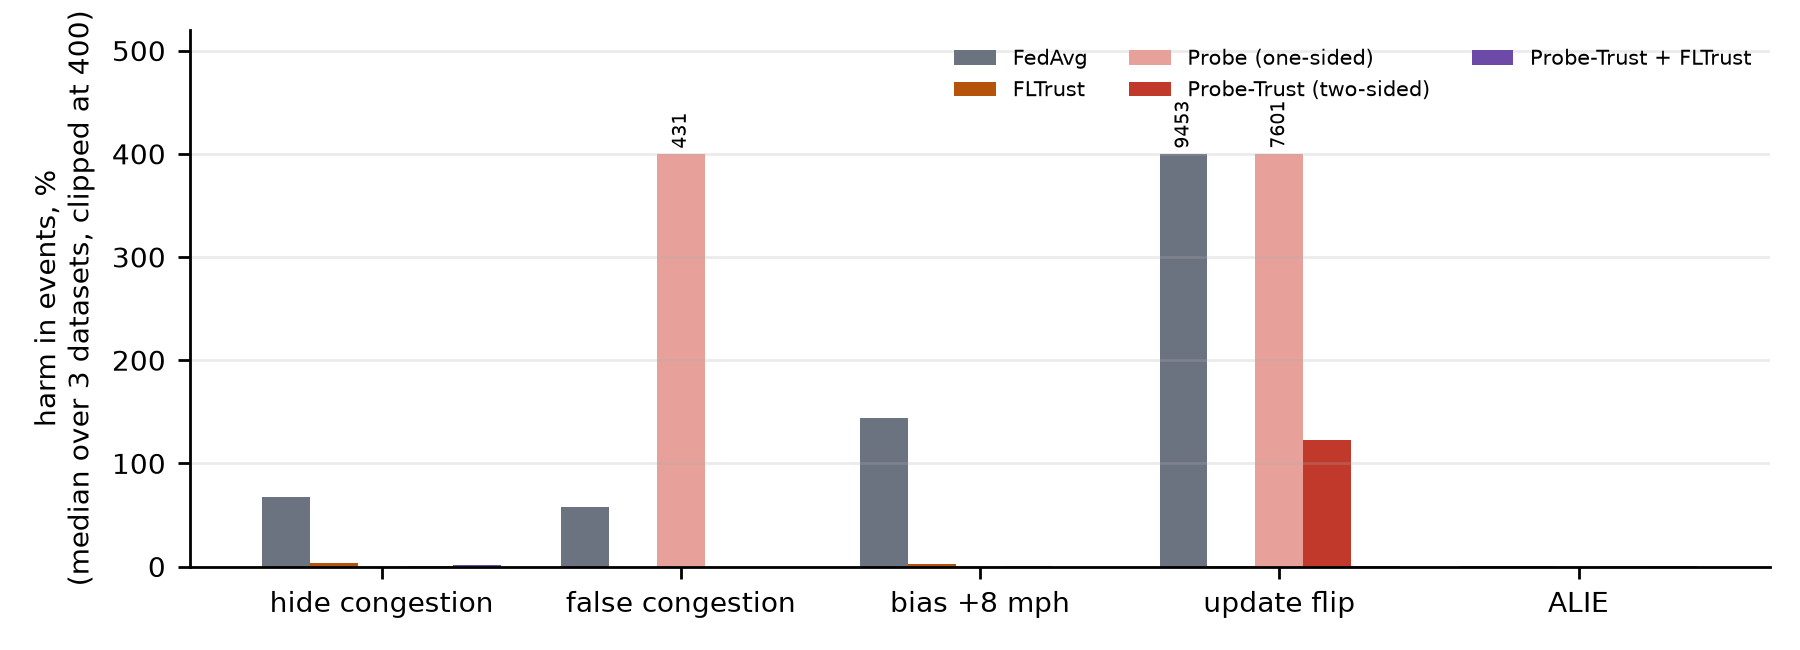
\includegraphics[width=15.5cm]{figs/fig_attacks40.png}
\caption{Harm in events at 40\% attackers by attack (median over three datasets, clipped at 400\%). The one-sided probe fails on false congestion and flip; two-sided Probe-Trust fails only on flip; combined with FLTrust it is close to zero everywhere.}
\end{figure*}
The remaining weaknesses are structural. Update flipping gives +123\% for the probes alone, because a flipped model can still produce plausible forecasts on the probes and the rule has no reference direction; with the FLTrust reference the combination reaches +0.1\%. Trigger backdoors are only partly reduced by the probes (median trigger shift 6.5 mph versus 10.6 mph for FedAvg at 40\%), and the combination with the root check removes them (0.0 mph). The harm of flipping falls from 40\% to 60\% attackers while that of FedAvg rises; we have no verified explanation and did not investigate it. Without attacks the weights cost nothing (harm -0.2\%).

\begin{figure*}[!t]
\centering
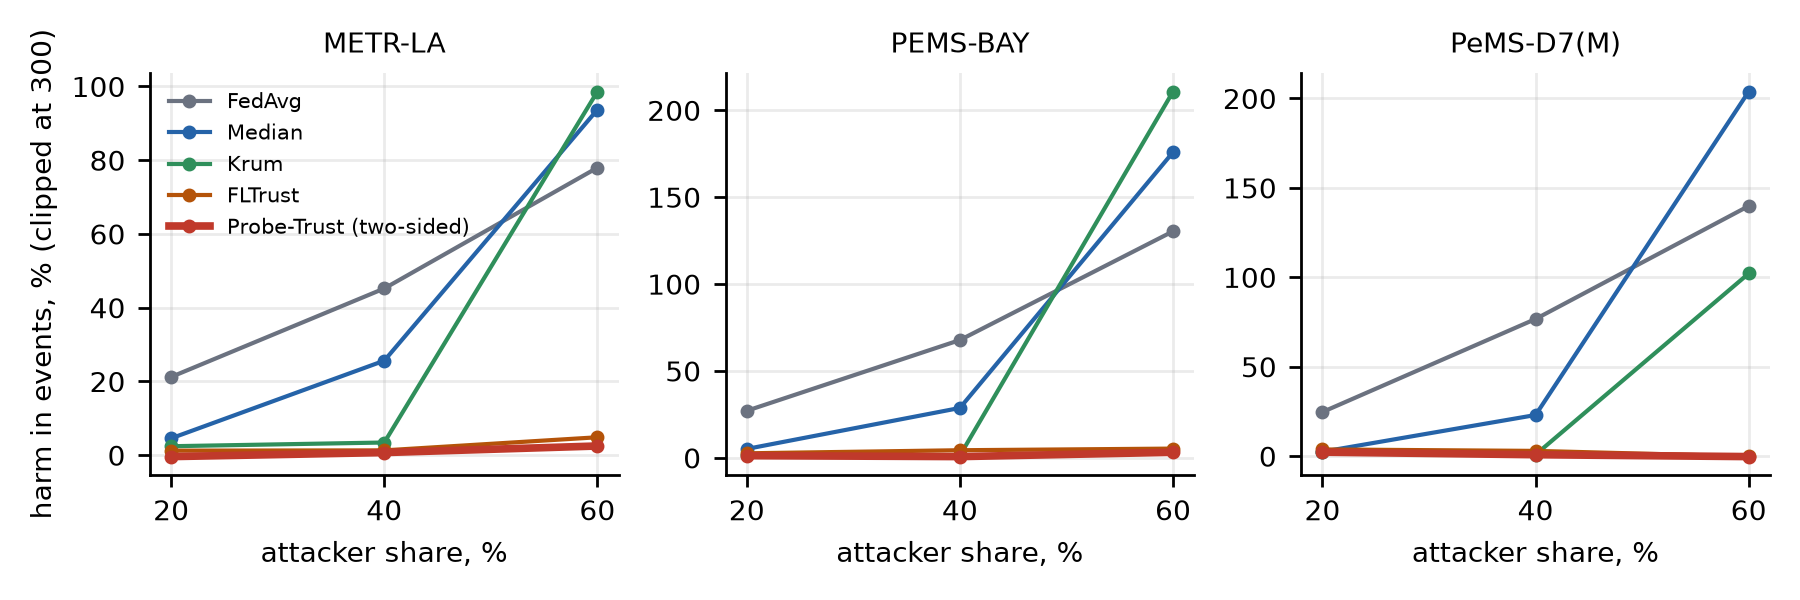
\includegraphics[width=15.5cm]{figs/fig_hide_share.png}
\caption{Harm in events versus the share of attackers for the hide attack. Probe-Trust stays near zero up to 60\%, while Krum with the true share breaks above 40\%.}
\end{figure*}
\subsection{Absolute versus cohort-relative scoring}
H1 attributes the operating range to the absolute form of the rule. We test this by an ablation that keeps the probes and changes only the scoring. In the cohort-relative variant the violation of each client is compared with the median and the median absolute deviation (MAD) of all clients, with a dead zone, in the style of \cite{uav} (the parameters of that work, \ensuremath{\beta} = 1 and dead zone 2, are used; this is our implementation of the scoring idea, not the authors' code). We add two cohort-based references written by us: a simplified FedMID-style rule \cite{fedmid} (random Gaussian inputs, relational distance matrices of the outputs, cohort outliers) and a FLAME-style rule \cite{flame} (HDBSCAN clustering of cosine distances, norm clipping, no noise). Table IV gives the harm in events. With 60\% attackers the relative variant of the same probes fails (+129.7 (+140.3) on hide, +229.4 (+505.3) on false congestion, +292.1 (+503.9) on bias), as do the FedMID-style, FLAME-style and Krum rules, while the absolute rule keeps +2.5 (+3.2), +0.8 (+1.4) and +2.2 (+6.2). Even at 40\% the relative variant is worse on bias (+16.2 (+35.7) against +0.4 (+3.8)). Cohort-relative scoring turns the attackers into the reference once they are the majority, which is the mechanism behind the honest-majority assumption. The FLAME-style rule, unlike the others, is the only one that handles update flipping at 40\% (+5.3\%) but fails at 60\% (+39448\%). H1 is therefore supported in the stronger form: the benefit comes from the absolute scoring, not from probing as such.

\begin{table*}[!t]
\caption{Ablation of the scoring rule: harm in events, \% --- median over datasets (worst dataset in parentheses); five seeds.}
\centering
\footnotesize
\renewcommand{\arraystretch}{1.12}
\begin{tabular}{|>{\raggedright\arraybackslash}p{6.67cm}|>{\raggedright\arraybackslash}p{0.94cm}|>{\raggedright\arraybackslash}p{2.72cm}|>{\raggedright\arraybackslash}p{2.72cm}|>{\raggedright\arraybackslash}p{2.72cm}|}
\hline
\textbf{Scoring rule} & \textbf{Share} & \textbf{Hide} & \textbf{False} & \textbf{Bias} \\
\hline
Probe-Trust (absolute rule) & 40\% & +0.7 (+0.8) & -0.3 (+0.4) & +0.4 (+3.8) \\
\hline
Probe-Trust (absolute rule) & 60\% & +2.5 (+3.2) & +0.8 (+1.4) & +2.2 (+6.2) \\
\hline
Same probes, cohort-relative (median/MAD) & 40\% & +6.6 (+10.1) & +0.5 (+0.8) & +16.2 (+35.7) \\
\hline
Same probes, cohort-relative (median/MAD) & 60\% & +129.7 (+140.3) & +229.4 (+505.3) & +292.1 (+503.9) \\
\hline
FedMID-style (random inputs, relational distances) & 40\% & +37.0 (+37.7) & +20.3 (+22.9) & +78.7 (+162.9) \\
\hline
FedMID-style (random inputs, relational distances) & 60\% & +127.4 (+133.5) & +223.9 (+804.2) & +570.4 (+826.1) \\
\hline
FLAME-style (cosine clustering) & 40\% & +52.9 (+58.9) & +0.6 (+9.1) & +1.5 (+20.5) \\
\hline
FLAME-style (cosine clustering) & 60\% & +116.2 (+143.3) & +524.7 (+817.1) & +605.8 (+867.5) \\
\hline
Krum (true share) & 40\% & +1.4 (+3.4) & -0.3 (+0.4) & +0.5 (+1.3) \\
\hline
Krum (true share) & 60\% & +102.1 (+210.8) & +524.5 (+822.9) & +606.2 (+867.0) \\
\hline
\end{tabular}
\end{table*}
\subsection{Dependence on clean server data (H3)}
We vary the root of FLTrust: 2 or 5 clients, one district (biased), a root with 3 of 10 poisoned clients, and non-IID clients (Table V, Fig. 3). With a clean root of 10 the difference to Probe-Trust is a few percentage points at most. With a poisoned root FLTrust degrades to +20.9\% (hide) and +16.0\% (bias) at 40\% attackers, whereas Probe-Trust remains at +1.0\% and +0.4\%. The criterion fixed in advance (interval of the paired difference below zero in at least two of three datasets) is applied to each scenario \ensuremath{\times} share cell; it is met in 9 of 12 hide cells and 7 of 12 bias cells and not met in the others, but the effect is of a few percentage points except with a poisoned root (about 15 points). For false congestion both are within about one point of zero; for flip Probe-Trust alone is worse. The combination with FLTrust inherits the root's weakness (+6.1\% and +10.2\% with the poisoned root). H3 is therefore supported in its weak form for non-adaptive attackers: Probe-Trust removes the need for trusted server data but does not outperform FLTrust with a good root; against a root-aware adaptive attacker the advantage is large (next subsection).

\begin{table*}[!t]
\caption{Harm in events, \%, at 40\% attackers by root scenario; left: hide, right: bias (median over datasets).}
\centering
\footnotesize
\renewcommand{\arraystretch}{1.12}
\begin{tabular}{|>{\raggedright\arraybackslash}p{4.35cm}|>{\raggedright\arraybackslash}p{1.55cm}|>{\raggedright\arraybackslash}p{1.55cm}|>{\raggedright\arraybackslash}p{2.35cm}|>{\raggedright\arraybackslash}p{1.55cm}|>{\raggedright\arraybackslash}p{1.55cm}|>{\raggedright\arraybackslash}p{2.35cm}|}
\hline
\textbf{Root scenario} & \textbf{FLTrust} & \textbf{Probe-Trust} & \textbf{Probe-Trust + FLTrust} & \textbf{FLTrust} & \textbf{Probe-Trust} & \textbf{Probe-Trust + FLTrust} \\
\hline
Clean root, 10 clients & +2.9 & +1.0 & +0.4 & +2.2 & +0.4 & -0.1 \\
\hline
Root of 2 & +1.9 & +1.0 & +0.8 & +5.5 & +0.4 & +0.3 \\
\hline
Root of 5 & +2.6 & +1.0 & +1.1 & +4.7 & +0.4 & +0.7 \\
\hline
Biased root (one district) & +5.2 & +1.0 & +0.3 & +4.9 & +0.4 & +0.7 \\
\hline
Poisoned root (3 of 10) & +20.9 & +1.0 & +6.1 & +16.0 & +0.4 & +10.2 \\
\hline
Non-IID clients & +3.7 & +0.6 & +1.2 & +1.7 & +0.3 & -0.0 \\
\hline
\end{tabular}
\end{table*}
\begin{figure*}[!t]
\centering
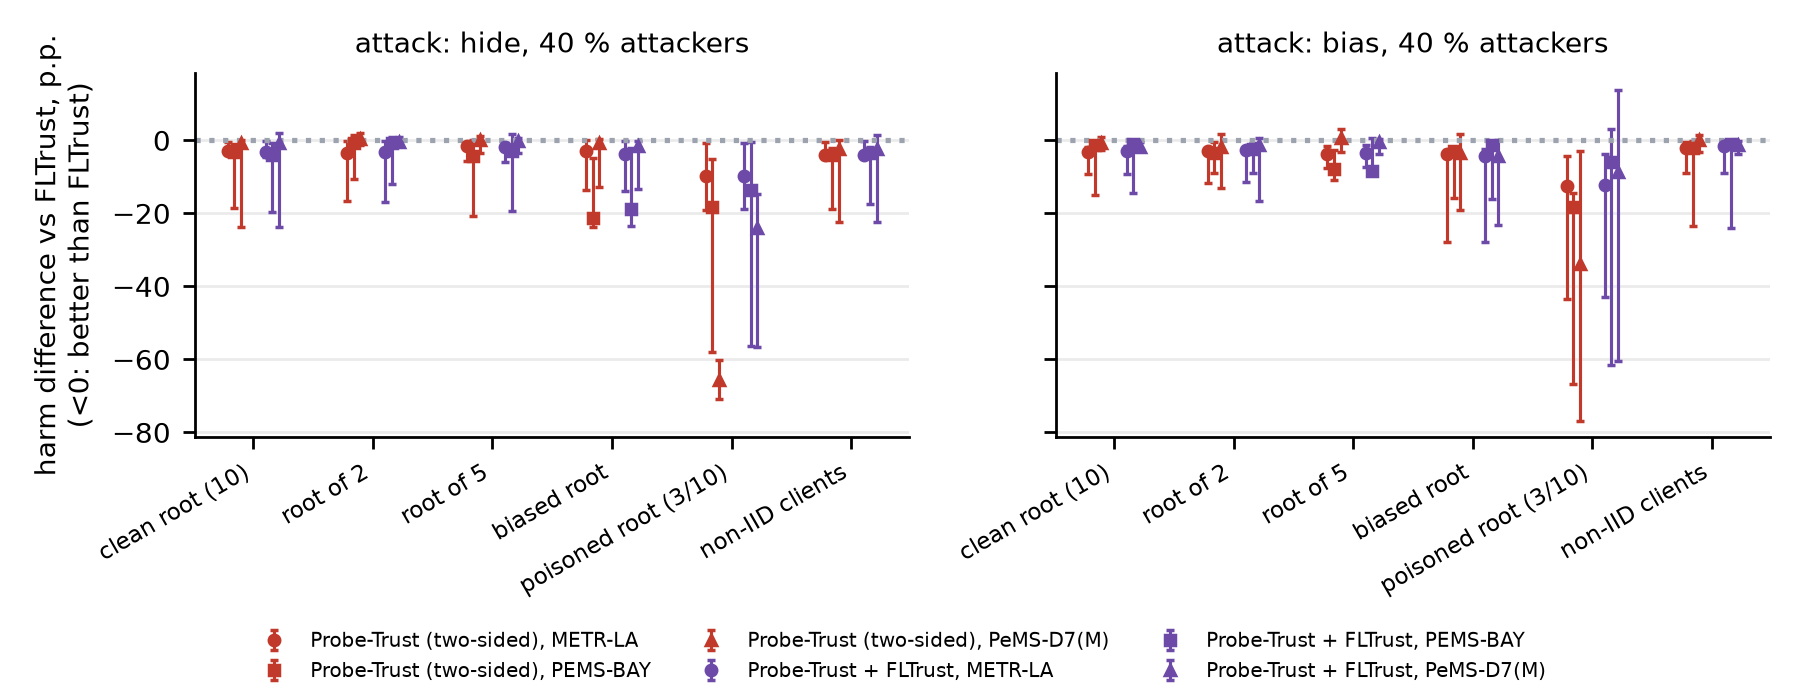
\includegraphics[width=15.0cm]{figs/fig_rootweak.png}
\caption{Paired difference of harm between Probe-Trust variants and FLTrust (percentage points, 95\% bootstrap interval over seeds, median over datasets). Negative values favour Probe-Trust.}
\end{figure*}
\subsection{Adaptive adversaries}
We also tested attackers that adapt to the defences (Table VI). Rule-compliant attackers train on their own probes (unknown to the server) or on the server's exact probes with a penalty for violating the rule; a root-aware attacker tunes its update to keep a fixed cosine similarity to the FLTrust root update; the last two rows combine them, without and with collusion. Attackers that obey the probe rule lose their power: their harm against Probe-Trust is bounded by +8.0\% at 60\% (and by +7.8\% against plain FedAvg). The root-aware attacker is the one that matters for H3: it raises the harm of FLTrust to +18.9\% (+24.2\% worst dataset) at 40\% and +29.5\% (+36.1\%) at 60\%, whereas Probe-Trust stays at +1.6\% and +3.5\% (worst dataset +7.4\%); the combination with FLTrust inherits part of the weakness (+8.4\% and +3.8\%). Collusion changes nothing measurable. Attackers that detect probes by input statistics were not evaluated.

\begin{table*}[!t]
\caption{Harm in events, \%, under adaptive attackers: median over datasets (worst dataset in parentheses); five seeds.}
\centering
\footnotesize
\renewcommand{\arraystretch}{1.12}
\begin{tabular}{|>{\raggedright\arraybackslash}p{5.15cm}|>{\raggedright\arraybackslash}p{0.95cm}|>{\raggedright\arraybackslash}p{2.05cm}|>{\raggedright\arraybackslash}p{2.05cm}|>{\raggedright\arraybackslash}p{2.15cm}|>{\raggedright\arraybackslash}p{2.75cm}|}
\hline
\textbf{Adaptive attacker} & \textbf{Share} & \textbf{FedAvg} & \textbf{FLTrust} & \textbf{Probe-Trust} & \textbf{Probe-Trust + FLTrust} \\
\hline
Trains on own probes, rule penalty & 40\% & +0.8 (+1.1) & +0.1 (+0.6) & +0.9 (+2.3) & -0.5 (+0.6) \\
\hline
Trains on own probes, rule penalty & 60\% & +1.8 (+4.5) & +0.4 (+1.5) & +1.6 (+4.5) & -0.0 (+2.1) \\
\hline
Trains on the server's exact probes & 40\% & +1.0 (+2.8) & +0.3 (+1.1) & +1.0 (+2.8) & -0.4 (+0.7) \\
\hline
Trains on the server's exact probes & 60\% & +1.5 (+7.8) & +1.5 (+2.1) & +1.9 (+8.0) & +0.8 (+2.0) \\
\hline
Root-aware (matches cosine to root update) & 40\% & +12.2 (+12.4) & +18.9 (+24.2) & +1.6 (+2.0) & +8.4 (+9.1) \\
\hline
Root-aware (matches cosine to root update) & 60\% & +23.2 (+25.6) & +29.5 (+36.1) & +3.5 (+7.4) & +3.8 (+10.5) \\
\hline
All of the above combined & 40\% & -0.5 (+0.6) & +0.1 (+1.2) & -0.9 (+0.4) & +0.1 (+0.7) \\
\hline
All of the above combined & 60\% & -0.1 (+1.5) & +0.9 (+2.8) & +1.3 (+2.2) & +0.6 (+3.4) \\
\hline
Combined + collusion (identical updates) & 40\% & -0.6 (+0.7) & -0.0 (+1.3) & -0.9 (+0.4) & +0.1 (+0.8) \\
\hline
Combined + collusion (identical updates) & 60\% & -0.2 (+1.5) & +1.0 (+1.8) & +0.9 (+2.3) & +0.3 (+3.4) \\
\hline
\end{tabular}
\end{table*}
\subsection{Attack strength, probe ranges, Min-Max and more seeds}
Attack strength (Table VII). The threshold \ensuremath{\delta} = 0.5\ensuremath{\sigma} is 6.4 mph, so a shift of 4 mph is inside the dead zone of the rule. There, Probe-Trust offers little protection: at 60\% attackers the harm of false congestion is +13.0\% (FedAvg +12.5\%, FLTrust +1.3\%) and that of bias +17.8\% (FedAvg +22.9\%, FLTrust +4.5\%), so a rule-compliant attacker keeps a harm of the order of the dead zone, and FLTrust with a clean root is better there. From 8 mph on, the harm falls to a few percent and does not grow with the shift, whereas FedAvg and the median grow with it. This bounds, empirically, what an attacker can gain without being detected by the probes; it is not a proof.

\begin{table*}[!t]
\caption{Harm in events, \% at 60\% attackers, by size of the attacker's shift (median over datasets; worst dataset in parentheses). Five seeds.}
\centering
\footnotesize
\renewcommand{\arraystretch}{1.12}
\begin{tabular}{|>{\raggedright\arraybackslash}p{2.35cm}|>{\raggedright\arraybackslash}p{1.55cm}|>{\raggedright\arraybackslash}p{2.75cm}|>{\raggedright\arraybackslash}p{2.75cm}|>{\raggedright\arraybackslash}p{2.75cm}|>{\raggedright\arraybackslash}p{2.75cm}|}
\hline
\textbf{Attack} & \textbf{Shift, mph} & \textbf{FedAvg} & \textbf{Median} & \textbf{FLTrust} & \textbf{Probe-Trust} \\
\hline
hide & 4 & +5.7 (+8.6) & +4.4 (+8.5) & +4.7 (+4.8) & +2.9 (+6.4) \\
\hline
hide & 8 & +23.3 (+27.9) & +24.7 (+31.2) & +5.4 (+7.7) & +7.4 (+12.9) \\
\hline
hide & 12 & +51.9 (+52.5) & +56.5 (+61.2) & +5.0 (+10.5) & +4.4 (+11.6) \\
\hline
false congestion & 4 & +12.5 (+28.6) & +24.2 (+57.3) & +1.3 (+3.8) & +13.0 (+28.5) \\
\hline
false congestion & 8 & +52.6 (+89.1) & +95.4 (+183.1) & +1.8 (+2.2) & +1.0 (+2.4) \\
\hline
false congestion & 12 & +98.9 (+143.9) & +177.1 (+318.5) & +1.5 (+1.8) & +1.0 (+1.4) \\
\hline
bias & 4 & +22.9 (+38.4) & +40.2 (+70.5) & +4.5 (+7.0) & +17.8 (+20.9) \\
\hline
bias & 8 & +65.7 (+97.1) & +128.6 (+207.5) & +4.2 (+7.7) & +6.0 (+6.1) \\
\hline
bias & 12 & +107.4 (+166.0) & +231.1 (+354.5) & +4.2 (+7.1) & +4.2 (+4.8) \\
\hline
\end{tabular}
\end{table*}
Misspecified probe ranges (Table VIII). The default ranges are q2--q10 for congestion and q60--q95 for free flow. More extreme ranges change little. Milder congestion probes, which are no longer in the regime in which the hide attack acts, break the protection against hiding: at 60\% the harm is +39.7\% on the median and +128.4\% on the worst dataset (PEMS-BAY). The method thus needs probes that really lie in the regime that attackers manipulate; this is a requirement on the domain knowledge, not a free parameter.

\begin{table*}[!t]
\caption{Two-sided Probe-Trust with misspecified probe ranges: harm in events, \% (median over datasets; worst dataset in parentheses). Five seeds.}
\centering
\footnotesize
\renewcommand{\arraystretch}{1.12}
\begin{tabular}{|>{\raggedright\arraybackslash}p{6.75cm}|>{\raggedright\arraybackslash}p{2.15cm}|>{\raggedright\arraybackslash}p{2.15cm}|>{\raggedright\arraybackslash}p{2.35cm}|>{\raggedright\arraybackslash}p{2.15cm}|}
\hline
\textbf{Probe range (percentiles of network speed)} & \textbf{Hide 40\%} & \textbf{Hide 60\%} & \textbf{False cong. 60\%} & \textbf{Bias 60\%} \\
\hline
congestion q0.5--q3, free flow q85--q99 (more extreme) & -0.6 (+0.5) & +0.7 (+2.0) & -0.1 (+1.4) & +7.1 (+10.4) \\
\hline
congestion q10--q25, free flow q40--q75 (milder) & +14.3 (+72.3) & +39.7 (+128.4) & +1.2 (+1.8) & +1.2 (+2.3) \\
\hline
\end{tabular}
\end{table*}
Min-Max and more seeds. The full-knowledge Min-Max attack \cite{minmax} is weak in this setting: at 60\% it gives +13.1\% for FedAvg, +6.2\% (+21.0\% worst dataset) for Probe-Trust and +2.8\% for FLTrust, while Krum and the median fail (+104\% and +90\%). For the key comparison at 60\% attackers we extended the runs from 5 to 20 seeds. Probe-Trust has harm +2.7\% (hide), +0.9\% (false congestion) and +1.8\% (bias); its paired difference to FLTrust is -3.7 [-5.2; -1.5], -0.7 [-1.0; -0.6] and -2.0 [-3.0; -0.4] percentage points (95\% bootstrap intervals over 60 paired dataset--seed runs). With a clean root the advantage over FLTrust is thus real but small, a few points. The cohort-relative variant with the same probes stays at +124\%, +228\% and +288\%, as in the five-seed ablation.

Probe-training attackers (Table IX). The attacker trains on probes of its own, either drawn like the server's or from a different family (other noise level, constant, slope and step shapes, wider ranges), and answers them with the honest last-speed value; the penalty weight punishes violations of the rule. Even so the attacker does not know the server's probes, and the two-sided check cannot be told from real windows by input statistics, which we did not test with a trained classifier. These attackers are weak against every method: at 60\% they cost plain FedAvg at most +7.4\% and Probe-Trust at most +7.7\% (worst dataset). The comparison therefore does not show robustness; it shows that mixing probes into the training data removes most of the attacker's own effect.

\begin{table*}[!t]
\caption{Harm in events, \% at 60\% attackers that train on their own probes: median over datasets (worst dataset in parentheses); five seeds.}
\centering
\footnotesize
\renewcommand{\arraystretch}{1.12}
\begin{tabular}{|>{\raggedright\arraybackslash}p{3.35cm}|>{\raggedright\arraybackslash}p{1.35cm}|>{\raggedright\arraybackslash}p{2.35cm}|>{\raggedright\arraybackslash}p{2.35cm}|>{\raggedright\arraybackslash}p{2.35cm}|>{\raggedright\arraybackslash}p{3.15cm}|}
\hline
\textbf{Attacker (own probes)} & \textbf{Penalty} & \textbf{FedAvg} & \textbf{FLTrust} & \textbf{Probe-Trust} & \textbf{Probe-Trust + FLTrust} \\
\hline
same family as server & 0 & +1.7 (+7.4) & +1.5 (+2.1) & +1.9 (+7.7) & +0.6 (+2.0) \\
\hline
same family as server & 5 & +1.7 (+5.7) & +0.6 (+1.8) & +1.8 (+7.0) & +0.0 (+2.0) \\
\hline
same family as server & 20 & +1.7 (+4.8) & +1.5 (+1.8) & +1.7 (+6.1) & +1.0 (+2.1) \\
\hline
different family & 0 & +1.9 (+3.1) & +1.4 (+2.1) & +2.5 (+2.8) & +0.4 (+2.0) \\
\hline
different family & 5 & +1.1 (+1.7) & +0.2 (+1.9) & +0.7 (+2.2) & -0.1 (+2.0) \\
\hline
different family & 20 & +1.0 (+1.5) & +1.5 (+1.7) & +0.5 (+2.1) & +1.2 (+1.9) \\
\hline
\end{tabular}
\end{table*}
Further attacks (Table X). The full-knowledge attack of Fang et al. \cite{fang}, which pushes each coordinate against the direction of the honest mean beyond the honest range, hurts FedAvg, the median and, at 60\%, Krum. Probe-Trust alone is only partly effective (+14.9\% at 40\% and +17.5\% at 60\%): the attack does not target the probe rule, so the probe check misses part of the damage, while FLTrust (+1.4\%) and the combination (+1.3\%) stay close to zero at 60\%. Scaling the poisoned update by ten (model replacement) is caught by Probe-Trust (+1.7\% at 60\% against FedAvg +731\%), and random noise does no measurable harm to any method. The combination with FLTrust is the safest choice over all attacks in this study.

\begin{table*}[!t]
\caption{Harm in events, \%: median over datasets; five seeds. Values of 100 or more are rounded.}
\centering
\footnotesize
\renewcommand{\arraystretch}{1.12}
\begin{tabular}{|>{\raggedright\arraybackslash}p{2.43cm}|>{\raggedright\arraybackslash}p{1.00cm}|>{\raggedright\arraybackslash}p{1.72cm}|>{\raggedright\arraybackslash}p{1.72cm}|>{\raggedright\arraybackslash}p{1.72cm}|>{\raggedright\arraybackslash}p{1.72cm}|>{\raggedright\arraybackslash}p{2.08cm}|>{\raggedright\arraybackslash}p{2.61cm}|}
\hline
\textbf{Attack} & \textbf{Share} & \textbf{FedAvg} & \textbf{Median} & \textbf{Krum} & \textbf{FLTrust} & \textbf{Probe-Trust} & \textbf{Probe-Trust + FLTrust} \\
\hline
Fang et al. & 40\% & +74.6 & +49.7 & +0.5 & +0.3 & +14.9 & +0.4 \\
\hline
Fang et al. & 60\% & +140 & +318 & +391 & +1.4 & +17.5 & +1.3 \\
\hline
Scale-up \ensuremath{\times}10 & 40\% & +380 & +20.9 & +0.5 & +6.8 & +1.1 & +0.0 \\
\hline
Scale-up \ensuremath{\times}10 & 60\% & +731 & +798 & +1.2 & +5.7 & +1.7 & +1.2 \\
\hline
Noise & 40\% & +0.8 & +0.6 & +0.1 & +0.5 & -0.3 & +0.2 \\
\hline
Noise & 60\% & +2.2 & +2.0 & +1.5 & +1.4 & +1.2 & +1.4 \\
\hline
\end{tabular}
\end{table*}
Zeno++ and FLAME (Table XI). We added two reference methods that reviewers asked for, both reimplemented from the papers because we found no official code for Zeno++ or FLAME \cite{zeno,flame}. Zeno++ clips each update to the norm of the server's own update and accepts it if its inner product with that update exceeds a fraction (0.1) of its squared norm; the threshold was not tuned. FLAME clusters the update directions with HDBSCAN, clips the norms to their median and adds noise of scale 0.001 times the median norm. At 60\% attackers the FLAME variants fail on all five attacks (+112\% on hide, +522\% on false congestion, +41337\% on flipping), because the largest cluster is the attackers, as expected without an honest majority. Zeno++ behaves like FLTrust: it stays within 6.7\% on all attacks, including flipping, which the probes alone do not stop. It uses a clean update on the server, like FLTrust, and on hide it is a few points behind Probe-Trust (+6.7\% against +2.5\%). This confirms the main limit of the work: when a trusted root is available, root-based rules are as good as the probes, and the probes are useful where it is not.

\begin{table*}[!t]
\caption{Harm in events at 60\% attackers, \%: median over three datasets and five seeds. Values of 100 or more are rounded.}
\centering
\footnotesize
\renewcommand{\arraystretch}{1.12}
\begin{tabular}{|>{\raggedright\arraybackslash}p{5.95cm}|>{\raggedright\arraybackslash}p{1.55cm}|>{\raggedright\arraybackslash}p{1.55cm}|>{\raggedright\arraybackslash}p{1.55cm}|>{\raggedright\arraybackslash}p{1.55cm}|>{\raggedright\arraybackslash}p{1.55cm}|}
\hline
\textbf{Method} & \textbf{Hide} & \textbf{False} & \textbf{Bias} & \textbf{Flip} & \textbf{ALIE} \\
\hline
Zeno++ (our reimplementation) & +6.7 & +1.8 & +4.8 & +2.4 & +2.9 \\
\hline
FLAME with noise (our reimplementation) & +112 & +522 & +606 & +41337 & +293 \\
\hline
FLAME-like, no noise & +106 & +522 & +606 & +40671 & +297 \\
\hline
FLTrust & +4.9 & +1.6 & +2.7 & +2.1 & +2.9 \\
\hline
Probe-Trust & +2.5 & +0.8 & +2.2 & +69.0 & +4.7 \\
\hline
\end{tabular}
\end{table*}
Stealth against strength (Table XII). An adaptive attacker that trains on probes mixes k probe windows into every local step; a larger k puts more weight on obeying the rule and, as a side effect, leaves less shift. We varied k from 4 to 48 for three attackers (the server's exact probes, the attacker's own probes, probes of a generic kind) without a penalty term, because the mixing itself is the lever. The table shows the expected trade-off: with few probe windows the attack is strong against FedAvg (+76.4\% at k = 4, 60\% attackers) and Probe-Trust holds it to +2.0\%; with many windows the attack is invisible to the probes, but it has also lost its effect even on FedAvg (+2.0\%). The worst harm of Probe-Trust over all attackers, k and shares is +10.9\% (worst dataset). The measured trade-off thus ends at a few percent, in line with the dead zone of the rule. As before, this is a test of three gradient-based attackers, not a proof for the best possible adversary.

\begin{table*}[!t]
\caption{Harm in events, \%, at 60\% attackers when the adaptive attacker mixes k probe windows into each local step (median over three datasets; five seeds; no penalty term).}
\centering
\footnotesize
\renewcommand{\arraystretch}{1.12}
\begin{tabular}{|>{\raggedright\arraybackslash}p{2.75cm}|>{\raggedright\arraybackslash}p{3.35cm}|>{\raggedright\arraybackslash}p{1.55cm}|>{\raggedright\arraybackslash}p{1.55cm}|>{\raggedright\arraybackslash}p{1.55cm}|>{\raggedright\arraybackslash}p{1.55cm}|}
\hline
\textbf{Attacker} & \textbf{Method} & \textbf{k = 4} & \textbf{k = 8} & \textbf{k = 16} & \textbf{k = 48} \\
\hline
exact server probes & FedAvg & +76.4 & +40.3 & +6.9 & +2.0 \\
\hline
exact server probes & FLTrust & +4.2 & +2.5 & +1.6 & +1.6 \\
\hline
exact server probes & Probe-Trust & +2.0 & +1.6 & +1.4 & +2.7 \\
\hline
exact server probes & Probe-Trust + FLTrust & +1.5 & +1.5 & +1.4 & +1.5 \\
\hline
own probes & FedAvg & +82.5 & +40.8 & +8.4 & +2.0 \\
\hline
own probes & FLTrust & +1.9 & +1.6 & +1.1 & +1.1 \\
\hline
own probes & Probe-Trust & +1.9 & +1.4 & +1.8 & +2.2 \\
\hline
own probes & Probe-Trust + FLTrust & +1.6 & +1.5 & +1.5 & +1.5 \\
\hline
generic probes & FedAvg & +81.6 & +44.3 & +6.0 & +2.5 \\
\hline
generic probes & FLTrust & +2.0 & +1.5 & +1.3 & +1.3 \\
\hline
generic probes & Probe-Trust & +2.1 & +1.5 & +1.3 & +3.0 \\
\hline
generic probes & Probe-Trust + FLTrust & +1.6 & +1.6 & +1.4 & +1.5 \\
\hline
\end{tabular}
\end{table*}
Strong non-IID data and other architectures (Table XIII). Two further robustness checks that reviewers asked for. First, nodes hold different, unequally sized subsets of windows (the non-IID option of our simulator); second, the whole experiment was repeated with a small transformer encoder, a three-layer perceptron and a graph-augmented GRU (the GRU receives a third input channel, the graph-weighted mean speed of the neighbouring sensors, i.e. one step of graph convolution; probes set this channel equal to the node's own speed) instead of the plain GRU, with the same thresholds (delta = 0.5\ensuremath{\sigma}, tau = 0.1\ensuremath{\sigma}) as elsewhere and no retuning. Probe-Trust stays at +2.8\% or less (median over datasets) in all 24 cells, while FedAvg loses between 61\% and 318\%, and the median and Krum fail at 60\%. FLTrust is clearly worse than on the GRU with the transformer (up to +11.6\%) and with the perceptron on bias at 60\% (+27.4\%), whereas Probe-Trust does not depend on the geometry of the updates. The cost on attack-free runs is -0.16\% (non-IID), -0.83\% (transformer) and -0.72\% (perceptron) for Probe-Trust, against +0.47\%, +0.78\% and -0.15\% for FLTrust. On the graph-augmented model FLTrust reaches +23.5\% (hide, 60\%) and the cost of Probe-Trust on clean runs is -0.49\%. The alternative architectures are small, and full spatio-temporal graph networks (STGCN, Graph WaveNet) were not tested.

\begin{table*}[!t]
\caption{Harm in events, \%, in four further conditions (median over three datasets; five seeds). Values of 100 or more are rounded.}
\centering
\footnotesize
\renewcommand{\arraystretch}{1.12}
\begin{tabular}{|>{\raggedright\arraybackslash}p{2.50cm}|>{\raggedright\arraybackslash}p{1.91cm}|>{\raggedright\arraybackslash}p{0.93cm}|>{\raggedright\arraybackslash}p{1.32cm}|>{\raggedright\arraybackslash}p{1.32cm}|>{\raggedright\arraybackslash}p{1.32cm}|>{\raggedright\arraybackslash}p{1.42cm}|>{\raggedright\arraybackslash}p{1.72cm}|>{\raggedright\arraybackslash}p{2.30cm}|}
\hline
\textbf{Condition} & \textbf{Attack} & \textbf{Share} & \textbf{FedAvg} & \textbf{Median} & \textbf{Krum} & \textbf{FLTrust} & \textbf{Probe-Trust} & \textbf{Probe-Trust + FLTrust} \\
\hline
Strong non-IID & hide & 40\% & +70.3 & +25.4 & +2.7 & +2.3 & +0.9 & +0.2 \\
\hline
Strong non-IID & hide & 60\% & +131 & +174 & +82.9 & +7.0 & +2.6 & +2.0 \\
\hline
Strong non-IID & false cong. & 40\% & +60.9 & +0.8 & -0.1 & +0.7 & -0.1 & +0.1 \\
\hline
Strong non-IID & false cong. & 60\% & +230 & +462 & +524 & +1.7 & +1.0 & +1.3 \\
\hline
Strong non-IID & bias & 40\% & +145 & +3.3 & +0.6 & +2.3 & +0.4 & +0.1 \\
\hline
Strong non-IID & bias & 60\% & +290 & +580 & +606 & +7.6 & +2.1 & +1.2 \\
\hline
Transformer & hide & 40\% & +87.8 & +73.0 & +15.9 & +9.5 & -0.2 & +0.7 \\
\hline
Transformer & hide & 60\% & +137 & +158 & +141 & +11.6 & -0.9 & -0.7 \\
\hline
Transformer & false cong. & 40\% & +171 & +3.0 & +1.4 & +6.3 & -0.3 & +0.8 \\
\hline
Transformer & false cong. & 60\% & +260 & +446 & +497 & +8.0 & -1.9 & -0.9 \\
\hline
Transformer & bias & 40\% & +221 & +19.4 & +1.4 & +8.8 & -0.2 & +0.9 \\
\hline
Transformer & bias & 60\% & +318 & +541 & +588 & +7.0 & -1.8 & -0.8 \\
\hline
MLP & hide & 40\% & +82.2 & +24.3 & +4.3 & +7.1 & -0.9 & -0.8 \\
\hline
MLP & hide & 60\% & +145 & +153 & +18.1 & +15.7 & +0.7 & +0.2 \\
\hline
MLP & false cong. & 40\% & +82.5 & +6.0 & -0.1 & +1.3 & -1.0 & -0.6 \\
\hline
MLP & false cong. & 60\% & +199 & +447 & +498 & +1.4 & +0.2 & -0.1 \\
\hline
MLP & bias & 40\% & +150 & +29.6 & -0.1 & +3.6 & -1.0 & -0.8 \\
\hline
MLP & bias & 60\% & +250 & +533 & +365 & +27.4 & +0.2 & -0.1 \\
\hline
Graph-augmented GRU & hide & 40\% & +69.0 & +45.8 & +9.8 & +8.0 & +1.4 & +2.4 \\
\hline
Graph-augmented GRU & hide & 60\% & +137 & +192 & +248 & +23.5 & +2.6 & +3.0 \\
\hline
Graph-augmented GRU & false cong. & 40\% & +111 & +4.3 & +1.1 & +3.9 & +0.2 & +1.1 \\
\hline
Graph-augmented GRU & false cong. & 60\% & +250 & +463 & +514 & +4.7 & +0.0 & +0.9 \\
\hline
Graph-augmented GRU & bias & 40\% & +123 & +12.8 & +1.1 & +3.8 & +1.5 & +1.1 \\
\hline
Graph-augmented GRU & bias & 60\% & +312 & +570 & +611 & +3.5 & +2.8 & +1.2 \\
\hline
\end{tabular}
\end{table*}
Can probes be told apart from real windows? (Table XIV). This is the main open question about any input-probing scheme: an adversary that detects probes can answer them honestly and misbehave on real inputs. We trained a gradient-boosting classifier (and a logistic regression) on 2000 probes and 2000 real windows from the training part of each network, with real windows restricted to the same last-speed range as the probes, and measured the AUC on 2000 new probes and 2000 real windows of the test part. The synthetic probes of the server are easy to detect: AUC 0.96--0.99, and 0.96 or more without range matching, because the noise of a probe is white while that of a sensor is not. An attacker with such a detector is a threat to the probe check that this paper does not rule out; the gradient-trained adaptive attackers above approximate it only partly, and with a perfect gate Probe-Trust reduces to FedAvg at the attacker share. As a mitigation we built probes from windows of the validation period of the same network (public history, no labels, only the last speed and the rule are used). Their detectability drops to AUC 0.60--0.78 for the boosting classifier (0.51--0.66 for the linear one); part of the remaining signal is the difference between periods, so this is an upper bound. The test is on one detector family and does not cover an attacker that adapts its detector to the server's probe generator over many rounds.

\begin{table*}[!t]
\caption{AUC of a classifier separating probes from real windows of the same last-speed range (gradient boosting; 0.5 = not separable).}
\centering
\footnotesize
\renewcommand{\arraystretch}{1.12}
\begin{tabular}{|>{\raggedright\arraybackslash}p{2.75cm}|>{\raggedright\arraybackslash}p{3.55cm}|>{\raggedright\arraybackslash}p{1.95cm}|>{\raggedright\arraybackslash}p{3.55cm}|>{\raggedright\arraybackslash}p{1.95cm}|}
\hline
\textbf{Dataset} & \textbf{Server's synthetic probes: congestion} & \textbf{free flow} & \textbf{Public-history probes: congestion} & \textbf{free flow} \\
\hline
METR-LA & 0.98 & 0.96 & 0.78 & 0.72 \\
\hline
PEMS-BAY & 0.99 & 0.99 & 0.73 & 0.60 \\
\hline
PeMS-D7(M) & 0.98 & 0.97 & 0.78 & 0.62 \\
\hline
\end{tabular}
\end{table*}
Protection with hard-to-detect probes (Table XV). Public-history probes keep the hide and false-congestion attacks at +2.8\% and +1.0\% at 60\% attackers and the adaptive attackers at +2.6\% and +1.9\% (worst dataset +11.1\%), but the bias attack is much less well handled (+24.9\% median and +55.3\% on the worst dataset, against +2.2\% with synthetic probes): with real windows, honest models also move on the probes, and the separation between honest and biased models is weaker. Combined with FLTrust the harm stays at +1.7\% or less, and the cost on clean runs is -0.1\%. There is therefore a trade-off between how well the probes can be hidden and how well they separate the models; the numbers for the synthetic probes in the earlier tables are an upper bound on the protection against an adversary that cannot detect probes.

\begin{table*}[!t]
\caption{Harm in events, \%, at 60\% attackers: synthetic probes of the paper and probes taken from public history of the same network (median over three datasets; worst dataset in parentheses; five seeds).}
\centering
\footnotesize
\renewcommand{\arraystretch}{1.12}
\begin{tabular}{|>{\raggedright\arraybackslash}p{3.61cm}|>{\raggedright\arraybackslash}p{1.68cm}|>{\raggedright\arraybackslash}p{3.03cm}|>{\raggedright\arraybackslash}p{3.42cm}|>{\raggedright\arraybackslash}p{4.00cm}|}
\hline
\textbf{Attack (60\% attackers)} & \textbf{FedAvg} & \textbf{Probe-Trust, synthetic probes} & \textbf{Probe-Trust, public-history probes} & \textbf{Probe-Trust + FLTrust, public-history probes} \\
\hline
hide & +130 & +2.5 & +2.8 (+4.8) & +1.7 \\
\hline
false congestion & +231 & +0.8 & +1.0 (+1.8) & +1.1 \\
\hline
bias & +292 & +2.2 & +24.9 (+55.3) & +0.9 \\
\hline
adaptive, exact probes & +53.8 & --- & +2.6 (+11.1) & +2.1 \\
\hline
adaptive, generic probes & +43.8 & --- & +1.9 (+3.6) & +1.5 \\
\hline
\end{tabular}
\end{table*}
A second domain: solar power forecasting (Table XVI). To test whether the idea is tied to traffic, we used the NREL Solar-Energy data distributed with LSTNet \cite{lstnet}: 137 photovoltaic plants in Alabama, 10-minute power for 2006, one client per plant, the same 12-step input and 3-step forecast, the same simulator and the same thresholds (delta = 0.5\ensuremath{\sigma}, tau = 0.1\ensuremath{\sigma}), without any tuning. Night values (zero) are treated as missing. The physical rule is the same: when the output is low, the forecast must not jump up by more than delta (a hidden shortfall), and when the output is high and steady it must not collapse (a false drop); probe ranges are the 2nd--10th and 60th--95th percentiles of the daytime output; events are midday (9:00--15:00) dips below 65\% of the typical output with at least three of four correlated neighbours also low. The attacks shift the labels by 20 MW (about 1.8\ensuremath{\sigma}) when the last output is below the 15th percentile (hide), above the median (false drop) or always (bias). Probe-Trust handles the false drop and bias attacks (-0.6\% and +0.9\% at 60\%, against +146\% and +299\% for FedAvg), but not the hide attack: +6.7\% at 40\% and +18.7\% at 60\%, no better than FedAvg (+6.2\% and +24.2\%). The weights separate the hide attackers from honest plants only partly (AUC 0.66 at 40\% and 0.92 at 60\%, against 0.99 for the false drop), so even a good ranking does not remove their influence; a plausible but untested reason is that honest forecasters also raise their forecast from a low output at sunrise and after clouds, so the rule is violated by honest models too. With the thresholds set after the fact, a tighter delta = 0.1\ensuremath{\sigma} lowers the harm of hide to +1.3\% and +3.9\% at a cost of +0.4\% on clean runs; this was chosen on the same data and is not an independent result. FLTrust and the combination handle all three attacks (at most +5.9\%). Only one dataset was used, so no between-dataset spread is available; the transfer is partial: the mechanism works where the rule is physically one-sided (a clear sky cannot produce a sudden surplus, a false drop is detectable) and needs a domain-specific design where the honest dynamics break the rule.

\begin{table*}[!t]
\caption{Solar power forecasting (137 plants): harm in events, \% (single dataset, five seeds). Thresholds as for traffic.}
\centering
\footnotesize
\renewcommand{\arraystretch}{1.12}
\begin{tabular}{|>{\raggedright\arraybackslash}p{3.42cm}|>{\raggedright\arraybackslash}p{0.91cm}|>{\raggedright\arraybackslash}p{1.49cm}|>{\raggedright\arraybackslash}p{1.49cm}|>{\raggedright\arraybackslash}p{1.49cm}|>{\raggedright\arraybackslash}p{1.59cm}|>{\raggedright\arraybackslash}p{1.97cm}|>{\raggedright\arraybackslash}p{2.65cm}|}
\hline
\textbf{Attack} & \textbf{Share} & \textbf{FedAvg} & \textbf{Median} & \textbf{Krum} & \textbf{FLTrust} & \textbf{Probe-Trust} & \textbf{Probe-Trust + FLTrust} \\
\hline
hide (low output) & 40\% & +6.2 & +1.3 & +1.0 & +0.2 & +6.7 & +0.4 \\
\hline
hide (low output) & 60\% & +24.2 & +61.3 & +96.2 & +1.7 & +18.7 & +1.9 \\
\hline
false drop (high output) & 40\% & +56.1 & +5.1 & -0.1 & +0.3 & -0.7 & -0.0 \\
\hline
false drop (high output) & 60\% & +146 & +322 & +391 & +5.9 & -0.6 & +1.3 \\
\hline
bias & 40\% & +168 & +10.4 & -0.2 & +0.2 & +0.3 & +0.0 \\
\hline
bias & 60\% & +299 & +598 & +623 & +1.4 & +0.9 & +1.3 \\
\hline
\end{tabular}
\end{table*}
\subsection{Absolute errors and trivial predictors}
Absolute errors and trivial predictors (Table XVII). Percentages of harm are relative to the clean RMSE, which is small on PEMS-BAY and PeMS-D7(M) (about 7 mph in events), so large percentages correspond to a few mph. More importantly, repeating the last observed speed is as accurate as the federated GRU in events (METR-LA 10.9 versus 12.4 mph; PEMS-BAY 7.1 versus 7.0; PeMS-D7(M) 7.2 versus 6.9) and clearly better on METR-LA, while the GRU is better over all windows. The compact model therefore has little forecasting skill beyond persistence at these horizons in events; the study measures the effect of poisoning on this model, not on a state-of-the-art forecaster.

\begin{table*}[!t]
\caption{RMSE in events on honest nodes, mph (median over seeds).}
\centering
\footnotesize
\renewcommand{\arraystretch}{1.12}
\begin{tabular}{|>{\raggedright\arraybackslash}p{2.13cm}|>{\raggedright\arraybackslash}p{1.58cm}|>{\raggedright\arraybackslash}p{1.76cm}|>{\raggedright\arraybackslash}p{1.76cm}|>{\raggedright\arraybackslash}p{1.94cm}|>{\raggedright\arraybackslash}p{1.94cm}|>{\raggedright\arraybackslash}p{2.13cm}|>{\raggedright\arraybackslash}p{1.76cm}|}
\hline
\textbf{Dataset} & \textbf{Persistence} & \textbf{Hist. average} & \textbf{FedAvg, clean} & \textbf{FedAvg, hide 40\%} & \textbf{FedAvg, hide 60\%} & \textbf{Probe-Trust, hide 60\%} & \textbf{Krum, hide 60\%} \\
\hline
METR-LA & 10.85 & 30.27 & 12.41 & 17.98 & 22.03 & 12.34 & 24.59 \\
\hline
PEMS-BAY & 7.13 & 27.66 & 7.01 & 11.77 & 16.17 & 7.24 & 21.81 \\
\hline
PeMS-D7(M) & 7.20 & 28.81 & 6.86 & 12.14 & 16.48 & 6.73 & 13.89 \\
\hline
\end{tabular}
\end{table*}
\subsection{Sensitivity to the thresholds}
Table XVIII varies \ensuremath{\delta} and \ensuremath{\tau} by a factor of two around the values used elsewhere (hide, false congestion and bias; three datasets; five seeds). Tightening either threshold does not increase the harm and costs nothing on clean data in this setting. Relaxing them raises the harm at 60\% attackers to +5.5\% (\ensuremath{\delta} = 1.0\ensuremath{\sigma}) and +3.2\% (\ensuremath{\tau} = 0.2\ensuremath{\sigma}) on the median, and to +16.0\% and +16.3\% on the worst dataset. The median harm therefore stays small under a twofold change of either threshold, but the worst dataset reaches 16\% when they are relaxed, so the thresholds should not be tuned loosely. Only \ensuremath{\delta} and \ensuremath{\tau} were varied; the speed ranges of the probes, which also come from network-level statistics, were not, and a setting with strongly non-IID honest clients may need smaller thresholds to avoid penalising honest nodes, which we did not test.

\begin{table*}[!t]
\caption{Sensitivity of two-sided Probe-Trust to \ensuremath{\delta} and \ensuremath{\tau}: harm in events, \% --- median over datasets and attacks (worst dataset in parentheses); cost on attack-free runs.}
\centering
\footnotesize
\renewcommand{\arraystretch}{1.12}
\begin{tabular}{|>{\raggedright\arraybackslash}p{1.88cm}|>{\raggedright\arraybackslash}p{1.88cm}|>{\raggedright\arraybackslash}p{4.39cm}|>{\raggedright\arraybackslash}p{4.39cm}|>{\raggedright\arraybackslash}p{3.23cm}|}
\hline
\textbf{\ensuremath{\delta} (in \ensuremath{\sigma})} & \textbf{\ensuremath{\tau} (in \ensuremath{\sigma})} & \textbf{40\%: median (worst dataset)} & \textbf{60\%: median (worst dataset)} & \textbf{Cost on clean data, \%} \\
\hline
0.25 & 0.1 & -0.5 (+2.4) & +1.2 (+4.5) & -0.33 \\
\hline
0.5 & 0.05 & -0.5 (+0.7) & +0.7 (+2.3) & -0.33 \\
\hline
0.5 & 0.1 & +0.4 (+3.8) & +1.5 (+6.2) & -0.24 \\
\hline
0.5 & 0.2 & +1.4 (+7.3) & +3.2 (+16.3) & -0.17 \\
\hline
1.0 & 0.1 & +1.9 (+5.8) & +5.5 (+16.0) & -0.13 \\
\hline
\end{tabular}
\end{table*}
\subsection{Limits}
(i) Thresholds do not transfer across datasets without normalisation (hence \ensuremath{\delta} and \ensuremath{\tau} in units of \ensuremath{\sigma}). (ii) Only small forecasters were evaluated (a GRU, a transformer encoder and a perceptron); graph-based models were not. (iii) Attackers that train on their own probes were tested and are weak against every method, but the synthetic probes are easy to tell from real windows (AUC above 0.95), so a detector-gated attacker is not excluded, and the probes that are hard to detect protect less against bias; attacks not bound by the rule's thresholds are not covered; Probe-Trust alone is also only partly effective against the Fang attack. (iv) Honest nodes are not demoted in the clean runs we examined: the 20\% of honest nodes with the most events in training receive a mean weight, relative to the mean over all nodes, of 1.16 (METR-LA), 1.02 (PEMS-BAY) and 1.01 (PeMS-D7(M)); we did not study the full distribution of honest weights, although the harm and the cost on clean runs under strongly non-IID clients are small (Section VI). (v) A learned defence selector based on server signals did not beat the best fixed rule on unseen networks (negative result, repository).

\section{Transfer to Ensembles of LLM Agents (H4)}
Setting. A coordinator receives 15-minute speed forecasts from ten LLM agents for one sensor and merges them. Agents run Qwen3-30B-A3B-Instruct-2507 \cite{qwen3} (4-bit, local, llama.cpp \cite{llamacpp}, temperature 0.6) with one of three role prompts and one of four sampling seeds (12 instances per pool). Real windows come from the METR-LA test split (40 event windows with mean target speed below 40 mph, 20 normal windows above 55 mph). A compromised agent receives a prompt-level override: hide (add 25 mph when the last speed is below 45 mph), false congestion (subtract 25 mph above 55 mph), or hide plus an instruction to answer honestly on inputs that look synthetic (probe-aware). The server sends four fixed probes (two congestion, two free flow) and applies Probe-Trust with the thresholds of Section IV (\ensuremath{\sigma} = 12.8 mph). Ensembles of ten are drawn at random from the pools (200 draws per window and share). Baselines: mean, median, trimmed mean, and an LLM coordinator (the same model reads the ten answers and returns a forecast). The plan and criteria were fixed before the main run; two size changes made for runtime (60 windows, shorter answer format) are documented.

\begin{table*}[!t]
\caption{LLM-agent ensembles: harm in events, \% (relative to a clean ensemble of ten honest agents) and AUC of the probe weights for separating compromised from honest agents. 40 event and 20 normal windows, 200 draws per window.}
\centering
\footnotesize
\renewcommand{\arraystretch}{1.12}
\begin{tabular}{|>{\raggedright\arraybackslash}p{2.15cm}|>{\raggedright\arraybackslash}p{0.95cm}|>{\raggedright\arraybackslash}p{1.45cm}|>{\raggedright\arraybackslash}p{1.45cm}|>{\raggedright\arraybackslash}p{1.45cm}|>{\raggedright\arraybackslash}p{1.65cm}|>{\raggedright\arraybackslash}p{2.05cm}|>{\raggedright\arraybackslash}p{1.85cm}|>{\raggedright\arraybackslash}p{0.85cm}|}
\hline
\textbf{Attack} & \textbf{Share} & \textbf{Mean} & \textbf{Median} & \textbf{Trimmed} & \textbf{LLM coord.} & \textbf{Probe (1-sided)} & \textbf{Probe-Trust} & \textbf{AUC} \\
\hline
hide & 40\% & +42.3 & +14.0 & +29.8 & +18.0 & +2.1 & +3.2 & 1.00 \\
\hline
hide & 60\% & +75.2 & +103.0 & +77.0 & +42.0 & +5.1 & +7.6 & 1.00 \\
\hline
exagg & 40\% & +315.8 & +11.1 & +250.0 & +6.9 & +0.4 & +0.6 & 1.00 \\
\hline
exagg & 60\% & +513.4 & +876.2 & +573.9 & +10.2 & +1.3 & +1.1 & 1.00 \\
\hline
hide aware & 40\% & +29.0 & +14.0 & +19.6 & +18.4 & +0.6 & +0.6 & 1.00 \\
\hline
hide aware & 60\% & +52.2 & +60.6 & +48.7 & +36.3 & +0.7 & +0.7 & 1.00 \\
\hline
\end{tabular}
\end{table*}
\begin{figure*}[!t]
\centering
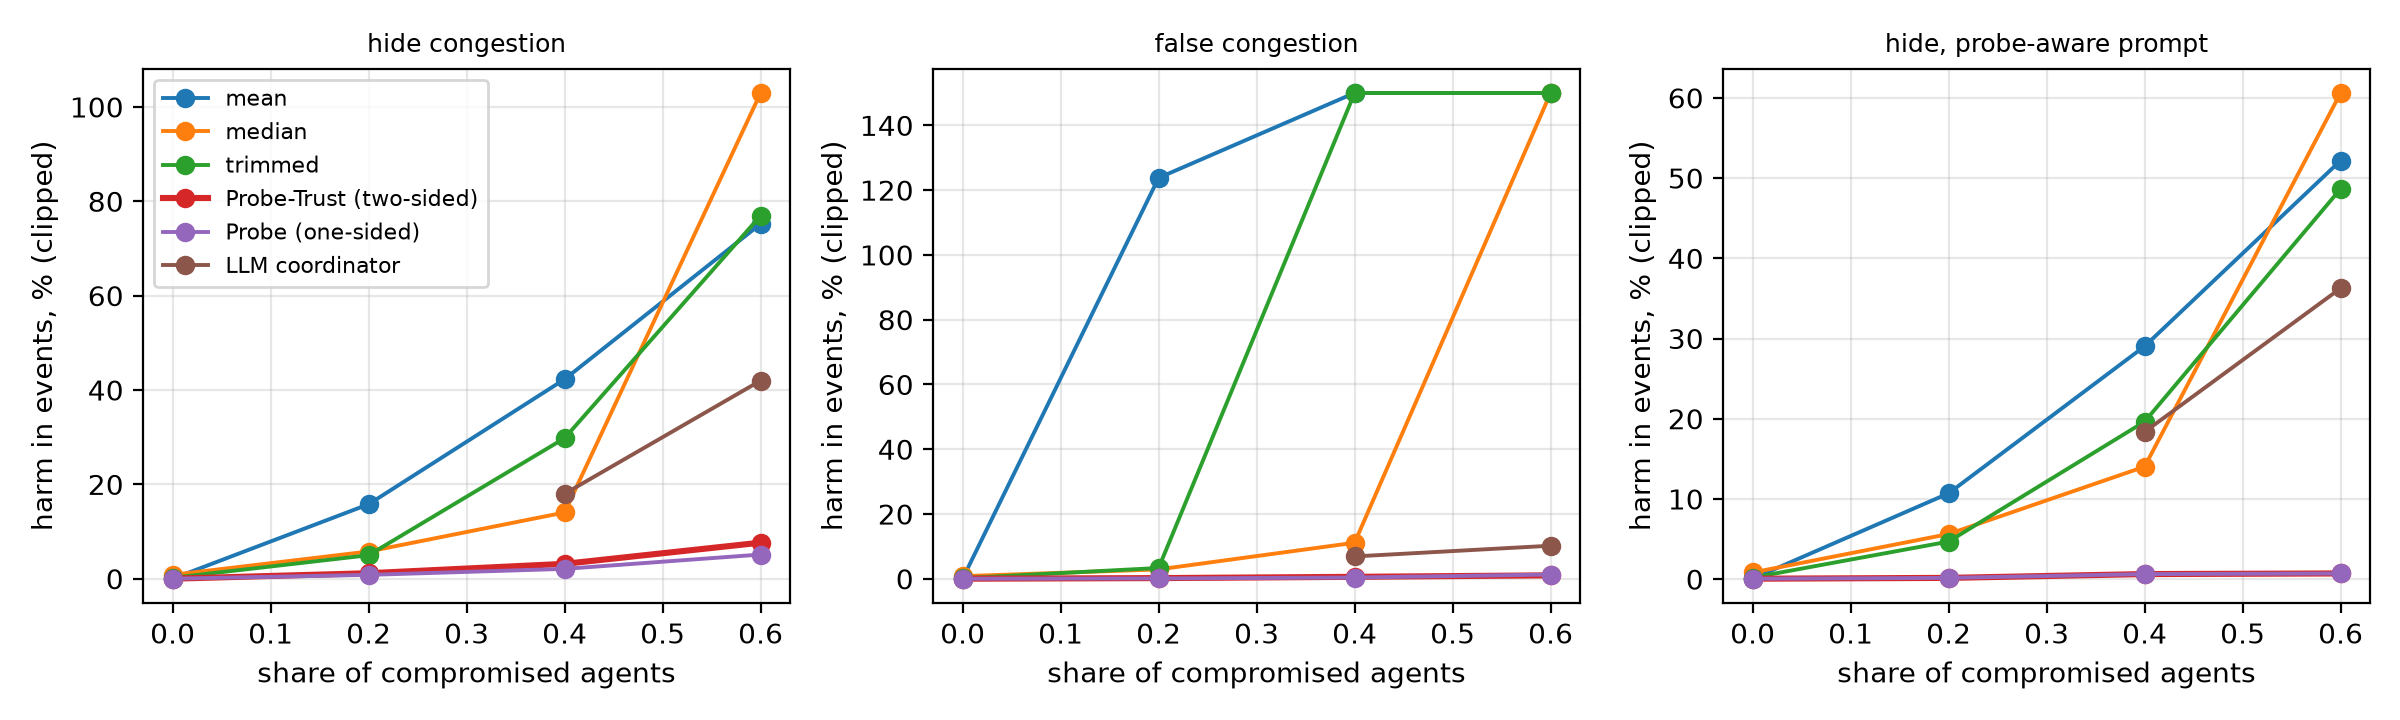
\includegraphics[width=16.0cm]{figs/fig_agentic.png}
\caption{LLM-agent ensembles: harm in events versus the share of compromised agents. Probe-Trust stays within a few percent; the median fails at 60\% and the LLM coordinator degrades with the share.}
\end{figure*}
Results. The attacks are effective (criterion C1): at 40\% the mean loses +42.3\% (hide) and +316\% (false congestion). The median fails at 60\% (+103\% and +876\%), where compromised agents form the majority; the LLM coordinator is better than the mean but not robust (+18.0\% at 40\% and +42.0\% at 60\% for hide). Probe-Trust keeps the harm at +3.2\% and +7.6\% (hide) and +0.6\% and +1.1\% (false congestion) at 40\% and 60\%, with no overhead on a clean ensemble (+0.0\%) and an AUC of 1.00 (C2, C4). The paired difference to the median at 60\% is -95 and -875 percentage points with intervals below zero (C3); against the LLM coordinator the interval at 60\% is below zero for false congestion and touches zero for hide in this run. H4 is therefore met for Qwen3-30B and not met for Mistral-7B (below).

What the experiment does not show. (i) An AUC of 1.00 reflects blunt overrides: compromised agents also drift on probes outside their trigger regime (under false congestion they raise the congestion probes from 22 to about 37 mph), so the one-sided probe suffices here, unlike in Section VI. (ii) The probe-aware prompt did not yield an adaptive adversary: the model could not recognise the probes as synthetic and applied the override to them even more strongly; this is not evidence of robustness against an engineered adversary. (iii) Two models, one task, 60 windows; the second model, below, gives weaker results, so this section is a preliminary study, not a validation. (iv) Probes had to be written by hand for the domain.

\begin{table*}[!t]
\caption{Weaker prompt overrides and a second model. Harm in events, \%, as in the previous table. Mistral-7B-Instruct-v0.3 (4-bit) could not follow the coordinator's answer format, so no LLM-coordinator result is available for it.}
\centering
\footnotesize
\renewcommand{\arraystretch}{1.12}
\begin{tabular}{|>{\raggedright\arraybackslash}p{2.15cm}|>{\raggedright\arraybackslash}p{2.55cm}|>{\raggedright\arraybackslash}p{1.15cm}|>{\raggedright\arraybackslash}p{1.75cm}|>{\raggedright\arraybackslash}p{1.75cm}|>{\raggedright\arraybackslash}p{2.15cm}|>{\raggedright\arraybackslash}p{0.95cm}|}
\hline
\textbf{Model} & \textbf{Attack} & \textbf{Share} & \textbf{Mean} & \textbf{Median} & \textbf{Probe-Trust} & \textbf{AUC} \\
\hline
Qwen3-30B & hide +25 (main) & 40\% & +42.3 & +14.0 & +3.2 & 1.00 \\
\hline
Qwen3-30B & hide +25 (main) & 60\% & +75.2 & +103.0 & +7.6 & 1.00 \\
\hline
Qwen3-30B & hide +10 & 40\% & +28.8 & +12.7 & +1.9 & 1.00 \\
\hline
Qwen3-30B & hide +10 & 60\% & +52.8 & +80.4 & +4.5 & 1.00 \\
\hline
Qwen3-30B & hide +5 & 40\% & +30.1 & +13.9 & +3.5 & 0.96 \\
\hline
Qwen3-30B & hide +5 & 60\% & +54.1 & +78.6 & +7.9 & 0.96 \\
\hline
Qwen3-30B & false cong. -10 & 40\% & +96.4 & +9.3 & +0.5 & 1.00 \\
\hline
Qwen3-30B & false cong. -10 & 60\% & +173.5 & +306.6 & +0.9 & 1.00 \\
\hline
Mistral-7B & hide & 40\% & +43.3 & +14.4 & +17.3 & 0.85 \\
\hline
Mistral-7B & hide & 60\% & +72.9 & +112.1 & +45.6 & 0.85 \\
\hline
Mistral-7B & false cong. & 40\% & +237.0 & +26.6 & +13.8 & 0.92 \\
\hline
Mistral-7B & false cong. & 60\% & +416.4 & +523.5 & +30.5 & 0.92 \\
\hline
Mistral-7B & hide, aware & 40\% & +64.6 & +14.2 & +17.1 & 0.85 \\
\hline
Mistral-7B & hide, aware & 60\% & +106.5 & +112.1 & +32.3 & 0.85 \\
\hline
\end{tabular}
\end{table*}
Weaker overrides and a second model. With smaller shifts (hide +10 and +5 mph, false congestion -10 mph) the probe weights still separate the compromised agents (AUC 1.00, 0.96 and 1.00), and Probe-Trust stays at +4.5\%, +7.9\% and +0.9\% at 60\%, against +52.8\%, +54.1\% and +173.5\% for the mean. A second model, Mistral-7B-Instruct-v0.3 (Apache-2.0), is clearly weaker: its answers are noisier (AUC of the weights only 0.85 for hide and 0.92 for false congestion), and Probe-Trust reaches +45.6\% (hide) and +30.5\% (false congestion) at 60\%. This is still lower than the mean (+72.9\% and +416.4\%) and the median (+112.1\% and +523.5\%), but it misses the criterion we set (harm of at most 10\% at 40\% and 60\%): at 40\% the harm is +17.3\% (hide) and the median is not worse than Probe-Trust (+14.4\%). We report this as a negative result for the weaker model: the absolute rule is robust to the share of attackers, but not to the noise of the honest agents, which the thresholds of Section IV were not tuned for.

Trivial baselines. A reviewer-style check is whether a rule without probes does as well. Clamping every agent's answer to within 0.5\ensuremath{\sigma} (6.4 mph) of the last observed speed and averaging (an absolute, cohort-free rule) gives, at 60\% compromised agents, -2.4\% (hide) and +103.0\% (false congestion) with Qwen3-30B, against +7.6\% and +1.1\% for Probe-Trust; with Mistral-7B it gives +14.2\% and +33.9\% against +45.6\% and +30.5\%. The clamp therefore beats Probe-Trust on the hide attack for both models and is comparable on false congestion for Mistral, but fails on false congestion for Qwen (+103.0\%): the clean error on normal windows is only 3.5 mph, so the residual shift of several mph that survives the clamp is a large relative harm there. Repeating the last observed speed, with no agents at all, is worse than the clean Qwen ensemble by +32.0\% and better than the Mistral ensemble (-2.7\%): the weaker model adds nothing over persistence, so the harm relative to its clean ensemble is a weak yardstick for it. We conclude that the LLM experiment shows that the probe weights detect blunt overrides, not that Probe-Trust is the best way to protect such an ensemble.

Two more models (Table XXI). We repeated the experiment with Llama-3.1-8B-Instruct and Gemma-2-9B-it (4-bit, same prompts and windows). Llama-3.1-8B did not follow the hidden override: the mean over its compromised ensemble is not harmed (-4.7\% for hide at 40\%), so the attack is ineffective and the model cannot test the defence; moreover Probe-Trust costs +31.7\% on the clean ensemble, because the honest answers of this model violate the probes (AUC of the weights 0.72). Gemma-2-9B answered 83\% of the real windows with an explanation instead of three numbers when honest, so for it we added one sentence to the prompt (``Do not explain and do not refuse...''), the same for all conditions; this deviates from the protocol used for the other models and its result is marked with an asterisk. With it, Gemma is attacked effectively (mean +28.0\% and +219.0\% at 40\%), and Probe-Trust handles the hide attack (harm +0.3\% and +0.9\% at 40\% and 60\%, AUC 1.00) but not false congestion (+75.3\% and +173.7\%), although the weights separate the agents perfectly (AUC 1.00); the weights of the compromised agents are too high to remove their influence with the thresholds fixed on the traffic simulator. Four further models, run later with the same protocol, agree with Qwen3-30B: Qwen2.5-14B-Instruct, Phi-4 and Gemma-2-27B-it are attacked effectively (mean harm +54\%, +30\% and +56\% for hide at 40\%), and Probe-Trust keeps the harm at 1.5\% or less in all four cells (AUC 0.99 or more). Mistral-Nemo-12B also needed the added sentence for its honest answers; with it, the attack works (mean +32\% and +189\%), Probe-Trust holds the harm at 4.0\% or less, but it costs +2.7\% on the clean ensemble. The LLM result is therefore model-dependent, but supported in most of the eight models: it is supported for Qwen3-30B, Qwen2.5-14B, Phi-4, Gemma-2-27B, Mistral-Nemo-12B (with a cost on clean data) and for hide with Gemma-2-9B; it is not supported for Mistral-7B and for false congestion with Gemma-2-9B, and not testable for Llama-3.1-8B.

\begin{table*}[!t]
\caption{Harm in events, \% for eight LLMs (ensemble of ten agents, shares of compromised agents as shown). *With an added sentence in the prompt (see text).}
\centering
\footnotesize
\renewcommand{\arraystretch}{1.12}
\begin{tabular}{|>{\raggedright\arraybackslash}p{2.62cm}|>{\raggedright\arraybackslash}p{2.04cm}|>{\raggedright\arraybackslash}p{1.85cm}|>{\raggedright\arraybackslash}p{2.62cm}|>{\raggedright\arraybackslash}p{1.85cm}|>{\raggedright\arraybackslash}p{2.62cm}|>{\raggedright\arraybackslash}p{1.66cm}|}
\hline
\textbf{Model} & \textbf{Attack} & \textbf{Mean 40\%} & \textbf{Probe-Trust 40\%} & \textbf{Mean 60\%} & \textbf{Probe-Trust 60\%} & \textbf{AUC 60\%} \\
\hline
Qwen3-30B & hide & +42.3 & +3.2 & +75.2 & +7.6 & 1.00 \\
\hline
Qwen3-30B & false cong. & +315.8 & +0.6 & +513.4 & +1.1 & 1.00 \\
\hline
Mistral-7B & hide & +43.3 & +17.3 & +72.9 & +45.6 & 0.85 \\
\hline
Mistral-7B & false cong. & +237.0 & +13.8 & +416.4 & +30.5 & 0.92 \\
\hline
Llama-3.1-8B & hide & -4.7 & +11.5 & -2.5 & +5.9 & 0.72 \\
\hline
Llama-3.1-8B & false cong. & -25.9 & -10.2 & -31.0 & -23.1 & 0.88 \\
\hline
Gemma-2-9B* & hide & +28.0 & +0.3 & +50.7 & +0.9 & 1.00 \\
\hline
Gemma-2-9B* & false cong. & +219.0 & +75.3 & +360.8 & +173.7 & 1.00 \\
\hline
Qwen2.5-14B & hide & +53.8 & +0.9 & +94.0 & +1.5 & 1.00 \\
\hline
Qwen2.5-14B & false cong. & +330.7 & +0.5 & +524.7 & +1.5 & 1.00 \\
\hline
Phi-4 (14B) & hide & +30.2 & +0.5 & +52.4 & +0.8 & 1.00 \\
\hline
Phi-4 (14B) & false cong. & +599.8 & +0.4 & +942.2 & +0.5 & 0.99 \\
\hline
Mistral-Nemo-12B* & hide & +31.7 & +3.1 & +56.3 & +4.0 & 0.99 \\
\hline
Mistral-Nemo-12B* & false cong. & +188.8 & +3.0 & +323.1 & +3.0 & 0.91 \\
\hline
Gemma-2-27B & hide & +56.2 & +0.1 & +99.6 & +0.6 & 1.00 \\
\hline
Gemma-2-27B & false cong. & +382.4 & +0.3 & +599.9 & +0.4 & 1.00 \\
\hline
\end{tabular}
\end{table*}
\section{Discussion}
Probe-Trust trades generality for verifiability: it needs a physical rule for the output on a controlled input. Where such a rule exists, it provides an absolute score that remains valid when attackers outnumber honest clients, which cohort-relative scoring \cite{uav} and distance-based rules cannot offer, and it needs no clean data, which root-of-trust defences \cite{fltrust,zeno} do. Against FLTrust with a good root, the measured gain is small; the practical value is robustness to the quality of the root and the freedom from trusted data. The probes are a form of known-answer testing and, for agents, of behavioural attestation: a participant is trusted to the extent that its answers on controlled inputs obey known constraints.

Limitations. The cohort-relative, FedMID-style, FLAME and Zeno++ variants are our own implementations, not the authors' code (we found none for Zeno++ and FLAME). We did not compare experimentally with generator-based or learned probing \cite{zafar,fedfg,specshield} or with learned reputation schemes \cite{rohfl,securegraphfl,flare,traftrust}, which address different tasks and have no released traffic implementation; the evidence is limited to the baselines of Table II. The physical rule must be specified per domain, probes that are indistinguishable from real inputs were not studied, and only small neural models and eight LLMs were used. Future work: graph forecasters, learned probe generation for other cyber-physical tasks, and engineered adaptive adversaries.

\section{Conclusion}
Rule-based probe windows give an absolute, label-free and cohort-free score of submitted forecasters. On three traffic datasets they keep the harm on honest nodes in events at +6.2\% or less with 60\% attackers on hide, false-congestion and bias attacks, require a two-sided rule, and remove the dependence on a clean root, but they do not stop update flipping or trigger backdoors without a root-based check. The guarantee is empirical and conditional: shifts below the dead zone of the rule (about 6 mph) are not prevented, and the probes must lie in the regime that attackers manipulate (milder congestion probes let the hide attack through). The same principle separated compromised LLM agents in a controlled numeric-consensus experiment. The probes are easy to tell from real windows, which leaves a detector-gated adversary open, and on solar power forecasting only two of the three attacks were stopped. The main open questions are engineered probe-aware adversaries and probes that are both hidden and discriminative, spatio-temporal graph forecasters, further domains, and a head-to-head comparison with learned probing.

\section*{Data and Code Availability}
Datasets are public (METR-LA, PEMS-BAY, PeMS-D7(M), and NREL Solar-Energy as distributed with LSTNet) and are not redistributed. Code, raw per-run logs, plans with success criteria, LLM answers and analysis scripts are in the repository https://github.com/asm0ra/probe-trust; sha256 checksums of the data files are listed there.


\begin{thebibliography}{99}
\bibitem{mcmahan} H. B. McMahan, E. Moore, D. Ramage, S. Hampson, and B. A. y Arcas, ``Communication-efficient learning of deep networks from decentralized data,'' in Proc. 20th Int. Conf. Artif. Intell. Statist. (AISTATS), 2017, pp. 1273--1282.
\bibitem{survey} C. Zhang, Y. Xie, H. Bai, B. Yu, W. Li, and Y. Gao, ``A survey on federated learning,'' Knowl.-Based Syst., vol. 216, Art. no. 106775, 2021, doi: 10.1016/j.knosys.2021.106775.
\bibitem{krum} P. Blanchard, E. M. El Mhamdi, R. Guerraoui, and J. Stainer, ``Machine learning with adversaries: Byzantine tolerant gradient descent,'' in Proc. Adv. Neural Inf. Process. Syst. (NeurIPS), vol. 30, 2017.
\bibitem{yin} D. Yin, Y. Chen, K. Ramchandran, and P. Bartlett, ``Byzantine-robust distributed learning: Towards optimal statistical rates,'' in Proc. 35th Int. Conf. Mach. Learn. (ICML), 2018, arXiv:1803.01498.
\bibitem{bulyan} E. M. El Mhamdi, R. Guerraoui, and S. Rouault, ``The hidden vulnerability of distributed learning in Byzantium,'' in Proc. 35th Int. Conf. Mach. Learn. (ICML), 2018, arXiv:1802.07927.
\bibitem{fltrust} X. Cao, M. Fang, J. Liu, and N. Z. Gong, ``FLTrust: Byzantine-robust federated learning via trust bootstrapping,'' in Proc. Netw. Distrib. Syst. Secur. Symp. (NDSS), 2021, doi: 10.14722/ndss.2021.24434.
\bibitem{zeno} C. Xie, S. Koyejo, and I. Gupta, ``Zeno++: Robust fully asynchronous SGD,'' in Proc. 37th Int. Conf. Mach. Learn. (ICML), 2020, arXiv:1903.07020.
\bibitem{flest} G. Geng, T. Cai, and Z. Yang, ``Better safe than sorry: Constructing Byzantine-robust federated learning with synthesized trust,'' Electronics, vol. 12, no. 13, Art. no. 2926, 2023, doi: 10.3390/electronics12132926.
\bibitem{fedmid} S. Han, H. Song, S. Park, and M. Cha, ``FedMID: A data-free method for using intermediate outputs as a defense mechanism against poisoning attacks in federated learning,'' arXiv:2404.11905, 2024.
\bibitem{danilenka} A. Danilenka, ``Tackling non-IID data and data poisoning in federated learning using adversarial synthetic data,'' J. Autom. Mobile Robot. Intell. Syst., 2024, doi: 10.14313/jamris/3-2024/17.
\bibitem{zafar} U. Zafar, A. M. H. Teixeira, and S. Toor, ``Byzantine-robust federated learning using generative adversarial networks,'' arXiv:2503.20884, 2025.
\bibitem{fedfg} R. Wang, R. Pan, and Z. Yao, ``FedFG: Privacy-preserving and robust federated learning via flow-matching generation,'' arXiv:2603.27986, 2026.
\bibitem{specshield} F. Hu, A. Zhang, M. Li, and C. Wang, ``Frequency-domain signatures for proactive defense against model poisoning attacks in federated learning,'' IEEE Trans. Inf. Forensics Security, 2026, doi: 10.1109/TIFS.2026.3689720.
\bibitem{uav} W. Jedrzejczak, C. Walther, D. Gill, and M. K. Hasan, ``Receiver-domain behavioral probing for backdoor-resilient federated GPS spoofing detection in UAV networks,'' arXiv:2610.10360, 2026.
\bibitem{normbound} Z. Sun, P. Kairouz, A. T. Suresh, and H. B. McMahan, ``Can you really backdoor federated learning?'' arXiv:1911.07963, 2019.
\bibitem{foolsgold} C. Fung, C. J. M. Yoon, and I. Beschastnikh, ``The limitations of federated learning in Sybil settings,'' in Proc. Int. Symp. Res. Attacks, Intrusions Defenses (RAID), 2020.
\bibitem{alie} G. Baruch, M. Baruch, and Y. Goldberg, ``A little is enough: Circumventing defenses for distributed learning,'' in Proc. Adv. Neural Inf. Process. Syst. (NeurIPS), 2019.
\bibitem{mudguard} R. Wang, X. Wang, H. Chen, J. Decouchant, et al., ``MUDGUARD: Taming malicious majorities in federated learning using privacy-preserving Byzantine-robust clustering,'' Proc. ACM Meas. Anal. Comput. Syst., 2024, doi: 10.1145/3700422.
\bibitem{securegraphfl} G. Chen, M. Tong, J. Yin, M. Wang, and J. Cao, ``SecureGraphFL: A privacy-preserving and attack-resilient federated learning framework for traffic prediction,'' IEEE Internet Things J., 2025, doi: 10.1109/JIOT.2025.3599568.
\bibitem{rohfl} H. Zhou, Y. Zheng, H. Huang, J. Shu, and X. Jia, ``Toward robust hierarchical federated learning in Internet of Vehicles,'' IEEE Trans. Intell. Transp. Syst., 2023, doi: 10.1109/TITS.2023.3243003.
\bibitem{wireless} Z. Zhang, M. Fang, J. Huang, and Y. Liu, ``Poisoning attacks on federated learning-based wireless traffic prediction,'' in Proc. IFIP Netw. Conf., 2024, doi: 10.23919/IFIPNetworking62109.2024.10619763.
\bibitem{flare} A. Younesi, L. Kiss, Z. N. Samani, J. A. Poveda, and T. Fahringer, ``FLARE: Adaptive multi-dimensional reputation for robust client reliability in federated learning,'' arXiv:2511.14715, 2025.
\bibitem{traftrust} T. Le Vinh, D. Le, H. T. Tran, and S. Bouzefrane, ``TrafTrust-Fed: Traffic-trust federated learning with fuzzy inference,'' IET Intell. Transp. Syst., 2026, doi: 10.1049/itr2.70234.
\bibitem{vettraffic} Q. Zhang, ``Revisiting the adversarial robustness of graph-based traffic forecasting,'' arXiv:2607.27604, 2026.
\bibitem{cpwbft} L. Zheng, J. Chen, Q. Yin, J. Zhang, X. Zeng, and Y. Tian, ``Rethinking the reliability of multi-agent system: A perspective from Byzantine fault tolerance,'' in Proc. AAAI Conf. Artif. Intell., 2026, arXiv:2511.10400.
\bibitem{sac} H. Lee, V.-D. Yun, D. Panagou, and S. P. Karimireddy, ``Robust multi-agent LLMs under Byzantine faults,'' in Proc. Conf. Empirical Methods Natural Lang. Process. (EMNLP), 2026, arXiv:2605.09076.
\bibitem{atrust} P. He et al., ``To trust or not to trust: Attention-based trust management for LLM multi-agent systems,'' in Proc. Annu. Meeting Assoc. Comput. Linguistics (ACL), 2026, arXiv:2506.02546.
\bibitem{springdrift} S. Brady, ``Springdrift: An auditable persistent runtime for LLM agents with case-based memory, normative safety, and ambient self-perception,'' arXiv:2604.04660, 2026.
\bibitem{trustprop} T. H. Safin, S. N. Zisad, S. Shatabda, and R. Hasan, ``Trust propagation and structural containment in multi-agent LLM pipelines,'' in Proc. IEEE Cyber Awareness Res. Symp. (CARS), 2026, arXiv:2609.17648.
\bibitem{rsmooth} J. Hu, Y. Dong, Z. Ding, and X. Huang, ``Enhancing robustness of LLM-driven multi-agent systems through randomized smoothing,'' Chin. J. Aeronaut., 2025, doi: 10.1016/j.cja.2025.103779.
\bibitem{snow} R. Snow, B. O'Connor, D. Jurafsky, and A. Y. Ng, ``Cheap and fast---but is it good? Evaluating non-expert annotations for natural language tasks,'' in Proc. Conf. Empirical Methods Natural Lang. Process. (EMNLP), 2008, doi: 10.3115/1613715.1613751.
\bibitem{dcrnn} Y. Li, R. Yu, C. Shahabi, and Y. Liu, ``Diffusion convolutional recurrent neural network: Data-driven traffic forecasting,'' in Proc. Int. Conf. Learn. Represent. (ICLR), 2018.
\bibitem{stgcn} B. Yu, H. Yin, and Z. Zhu, ``Spatio-temporal graph convolutional networks: A deep learning framework for traffic forecasting,'' in Proc. 27th Int. Joint Conf. Artif. Intell. (IJCAI), 2018, doi: 10.24963/ijcai.2018/505.
\bibitem{flame} T. D. Nguyen, P. Rieger, H. Chen, H. Yalame, et al., ``FLAME: Taming backdoors in federated learning,'' in Proc. 31st USENIX Security Symp., 2022, arXiv:2101.02281.
\bibitem{minmax} V. Shejwalkar and A. Houmansadr, ``Manipulating the Byzantine: Optimizing model poisoning attacks and defenses for federated learning,'' in Proc. Netw. Distrib. Syst. Secur. Symp. (NDSS), 2021.
\bibitem{fang} M. Fang, X. Cao, J. Jia, and N. Gong, ``Local model poisoning attacks to Byzantine-robust federated learning,'' in Proc. USENIX Security Symp., 2020.
\bibitem{lstnet} G. Lai, W.-C. Chang, Y. Yang, and H. Liu, ``Modeling long- and short-term temporal patterns with deep neural networks,'' in Proc. 41st Int. ACM SIGIR Conf. Res. Develop. Inf. Retrieval, 2018, pp. 95--104.
\bibitem{qwen3} A. Yang et al., ``Qwen3 technical report,'' arXiv:2505.09388, 2025.
\bibitem{llamacpp} G. Gerganov et al., ``llama.cpp: LLM inference in C/C++,'' GitHub repository, https://github.com/ggml-org/llama.cpp.
\end{thebibliography}
\end{document}
